\documentclass[11pt]{book}

\usepackage{fullpage}
\usepackage{graphicx}
\usepackage{cite}
\usepackage{times}
\usepackage{url}
%%\usepackage{hyperref}
\usepackage{setspace}
\usepackage{fancyhdr}
\usepackage{ifthen}
\usepackage{listings}
\usepackage{color}
\usepackage[section]{placeins}
\usepackage{xtab}
\usepackage{url}
\usepackage[space]{grffile}
\usepackage[ruled]{algorithm2e}
\usepackage{float}

\setcounter{topnumber}{2}
\setcounter{bottomnumber}{3}
\setcounter{totalnumber}{4}
\renewcommand{\topfraction}{0.5}
\renewcommand{\bottomfraction}{0.95}
\renewcommand{\textfraction}{0.1}
\renewcommand{\floatpagefraction}{0.7}

\setlength{\abovecaptionskip}{3pt}
\setlength{\belowcaptionskip}{3pt}

\pagestyle{fancy}
\setboolean{@twoside}{false}
\setlength{\headsep}{25pt}
\setlength{\headheight}{14pt}

\newcommand{\showPlots}[3]{
  \begin{figure}
    \begin{minipage}{.5\textwidth}
      \begin{center}
        \includegraphics[width=\textwidth,keepaspectratio]{figs/traffic/#1} \\
        Traffic Model \\
      \end{center}
    \end{minipage} \hfill
    \begin{minipage}{.5\textwidth}
      \begin{center}
        \includegraphics[width=\textwidth,keepaspectratio]{figs/pcs/#1} \\
        PCS Model \\
      \end{center}
    \end{minipage}
    \begin{minipage}{.5\textwidth}
      \begin{center}
        \includegraphics[width=\textwidth,keepaspectratio]{figs/epidemic/#1} \\
        Epidemic Model \\
      \end{center}
    \end{minipage} \hfill
    \begin{minipage}{.5\textwidth}
      \begin{center}
        \includegraphics[width=\textwidth,keepaspectratio]{figs/airport/#1} \\
        Airport Model \\
      \end{center}
    \end{minipage}
    \caption{#3}\label{#2}
  \end{figure}
}

\definecolor{dkgreen}{rgb}{0,0.6,0}
\definecolor{gray}{rgb}{0.5,0.5,0.5}
\definecolor{mauve}{rgb}{0.58,0,0.82}

\lstset{frame=tb,
  language=C++,
  columns=flexible,
  basicstyle={\linespread{0.9}\small\ttfamily},
  breaklines=true,
  captionpos=b,
  aboveskip=0.2in,
  belowskip=0.2in,
  numberstyle=\tiny\color{gray},
  keywordstyle=\color{blue},
  commentstyle=\color{dkgreen},
  stringstyle=\color{mauve},
  tabsize=4
}

\begin{document}

\thispagestyle{empty}

\doublespacing

\vspace*{0.5in}

\begin{center}
\LARGE{\textbf{Time Warp Simulation on Multi-core Processors and Clusters}}

\vspace*{0.4in}

  {\large A thesis submitted to the\\[0.20in]
    Division of Research and Advanced Studies\\
    of the University of Cincinnati\\[0.20in]
    in partial fulfillment of the\\
    requirements for the degree of\\[0.20in]
    \textbf{MASTER OF SCIENCE}\\[0.20in]
    in the School of Electric and Computing Systems\\
    of the College of Engineering and Applied Sciences\\[0.20in]
    August xx, 2015\\[0.20in]
    by\\[0.20in]
    \textbf{Doug Weber}\\
    BSEE, University of Cincinnati, 2014\\}
  \vspace{0.5in}
  {\large Thesis Advisor and Committee Chair:  Dr. Philip A. Wilsey}
\end{center}

\clearpage

\setcounter{page}{1}
\pagenumbering{roman}
\clearpage

\chapter*{Abstract}

%% the abstract covers your thesis soup to nuts.  the abstract may be published
%% separately from the main body so it needs to be fully contained and say
%% something about nearly everything in your thesis.  basically in 1-2 pages you
%% need to: bring the reader into your topic, explain why it is important and
%% why existing solutions are insufficient, it must describe your approach to a
%% solution and what your primary results are.  whew!!



\chapter*{Acknowledgments}



\tableofcontents \markright{ }
\listoffigures \markright{ }
%\listoftables \markright{ }
\listofalgorithms \markright { }
\lstlistoflistings \markright{ }

\clearpage
\pagenumbering{arabic} \setcounter{page}{1}

\chapter{Introduction}\label{intro}

\section{Motivation and Plan of Study}

%% Background
Many systems can be described by events that occur in discrete time intervals such as
communication networks, digital logic circuits, transportation systems, or disease
outbreak. To gain a better understanding of these systems, researchers develop models of
the systems and perform simulations on computing platforms. These \emph{Discrete Event
Simulations} (DESs) can take a long time to simulate large, complex systems by sequentially
processing events and has led researchers to design parallel algorithms to run simulations
on parallel computing platforms. The field of study that deals with parallel algorithms
to speed up discrete event simulations is called Parallel Discrete Event Simulation (PDES).

Parallel algorithms can be written for shared memory architectures, clusters, or any other
type of system that supports hardware concurrency. Furthermore, communication between
concurrent workers in the system can be achieved through shared data structures or through
explicit messages that are passed among workers.

%% Problem Statement
Some time warp systems are designed for only shared memory multiprocessors and use shared
memory for communication. Thes systems minimize communication latencies and allow very fast,
simple algorithm because everything can run in a single address space and use shared data
structrures but are still limited in computational power, memory size, and memory bandwidth.

Other time warp systems are completely based on a message passing system that can be scaled
to any number of processor cores on any number of machines. However, the time it takes to
exchange messages with message passing is usually higher due to message copying, temporary
buffering, and network latencies.

%% Solution
The \textsc{warped2} simulation kernel, which is a reimplementation of the original
\textsc{warped} simulation kernel, is an entirely different approach which uses shared
memory between \emph{worker threads} in a single process to eliminate communication overheads,
but uses message passing between processes to allow the system to scale to larger sizes.
A dedicated \emph{manager thread} handles all message passing communication between processes.
Figure \ref{warped2_communication} illustrates the communication model that is used in
\textsc{warped2}.

\begin{figure}[H]
    \centering
    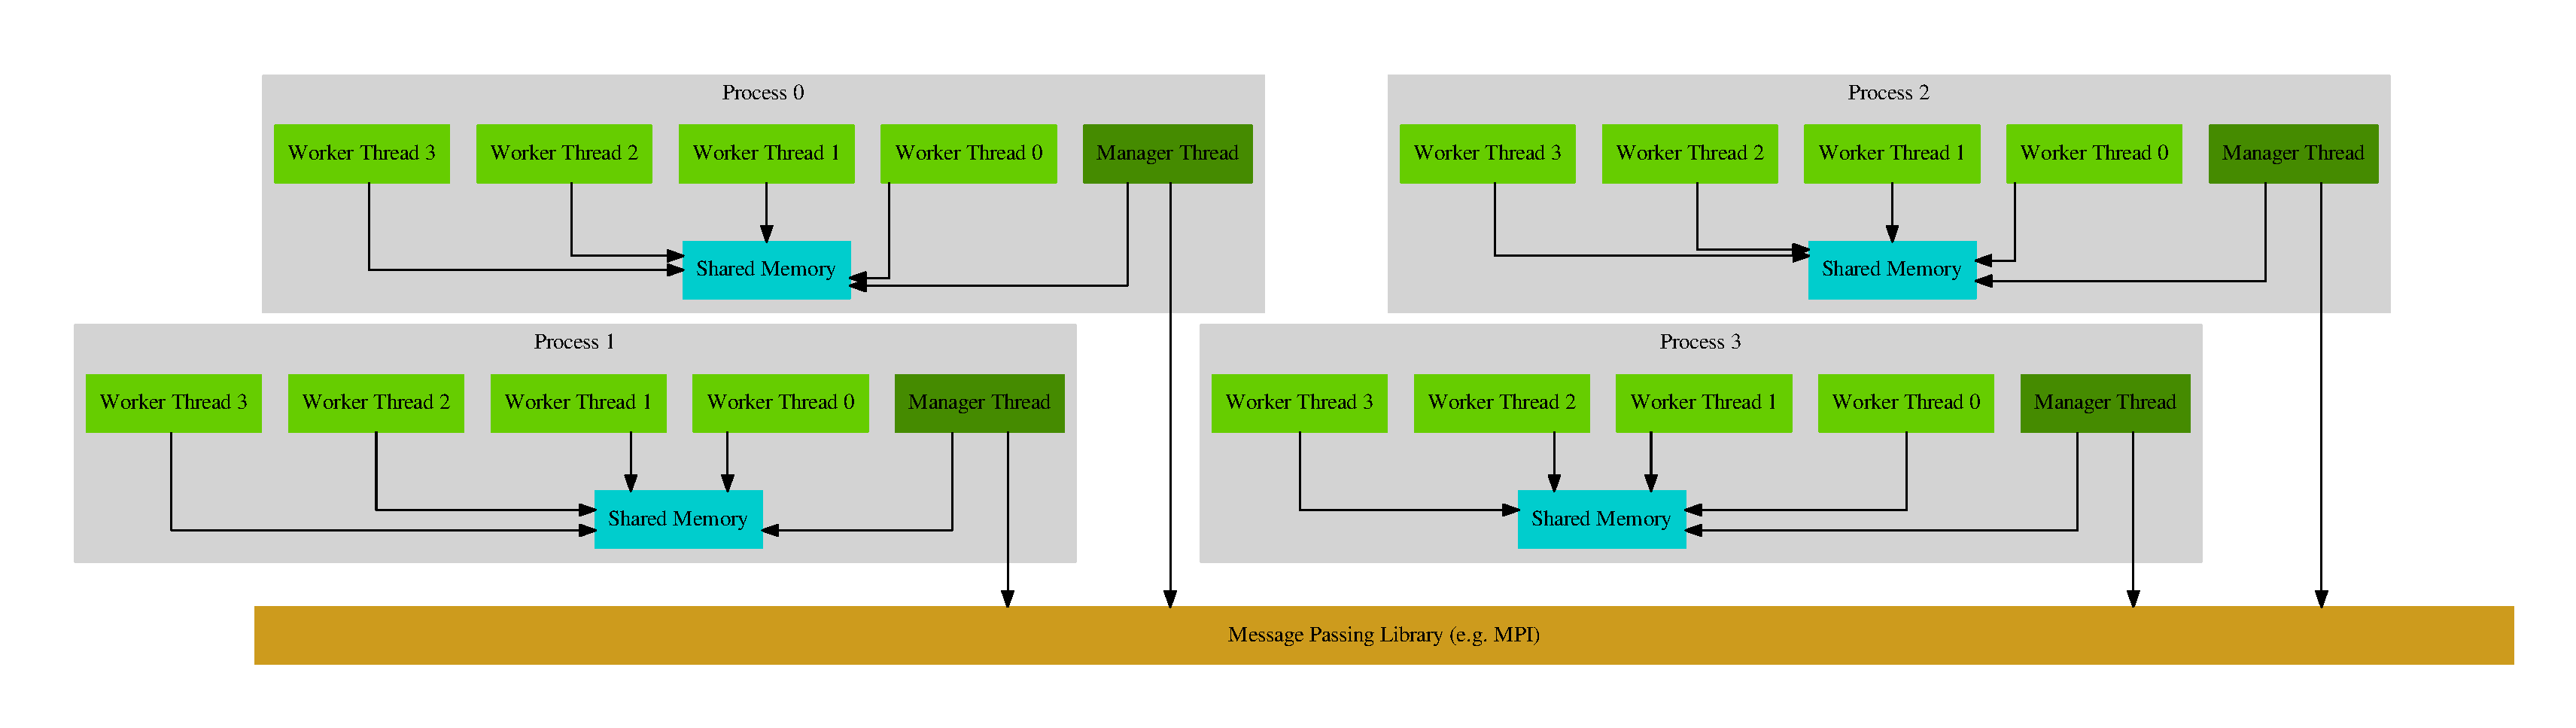
\includegraphics[width=\textwidth]{figs/graphviz/warped_communication.pdf}
    \caption{Communication Model of \textsc{warped2}}\label{warped2_communication}
\end{figure}

%% Scheduling
This communication model not only allows for high scalability and reduced communication
overhead within processeses, but allow the simulation to follow the critical path better
since the worker threads can share a scheduling data structure to process events from.
Less scheduling data structures creates a bottleneck since multiple worker threads cannot
access them simultaneously without race conditions. On the other hand, more scheduling
data structures allows more concurrency but spreads out the critical path of execution,
allowing more rollbacks.

%% Partitioning
To further reduce any communication overheads in both message passing and shared memorory
communication, partitioning the work between processes can have a significant impact.
Partitioning the work between processes in a parallel discrete event simulation can be
achieved by partitioning the logical processes 

%% GVT and Termination
The combination of shared memory and message passing communication does create some
complications in the implementation of a time warp system. GVT and termination detection
algorithms are usually designed for either shared memory or message passing but not both.
Using a single message passing algorithm between worker threads and processes would mean
that some kind of message passing scheme would have to be implemented for worker threads
to communicate. This scheme would still use shared memory for message communication but
would still have the overheads of using explicit messages. On the contraray, it is possible
to have a single shared memory algorithm that extends to distributed memory systems but
would require shared virtual memory. A shared virtual memory system would still have to
transparently use message passing to achieve synchronization. For these reasons, the
GVT and termination algorithms developed for \textsc{warped2} include a message passing
base algorithm and a shared memory subalgorithm.

%% Shared Memory
Using shared memory introduces a whole new set of problems that must be 

\section{Thesis Overview}

The remainder of this thesis is organized as follows:

Chapter \ref{background} contains some background information on parallel simulation and
parallel computing that is used in this thesis.

Chapter \ref{related_work} reviews several of the prominent parallel simulation kernels
that use the Time Warp synchronization protocol.  The software architecture and target
compute platforms for each is described.

Chapter \ref{warped2_overview} introduces the software architecture and modeling API for
the \textsc{warped2} simulation kernel.

Chapter \ref{plans_of_study} gives an overview of the studies carried out in the remainder
of the text, motivations for the studies, and the hardware architectures and simulation
models used in the studies.

Chapter \ref{warped2_ds} describes the pending event set data structures used within
the \textsc{warped2} kernel and provides some preliminary results in finding the best
configurations for various models.

Chapter \ref{partitioning} talks about partitioning.

Chapter \ref{gvt_termination} descibes various GVT and termination detection algorithms that
have been used explains the algorithms used in \textsc{warped2}. This chapter also provides
some preliminary results in determining the best configurations for these algorithms.

Chapter \ref{memory_management} analyzes techniques for managing memory efficiently. This
includes state saving techniques, fossil collection, and GVT period. Some preliminary results
are also shown for various configurations.

Chapter \ref{results_summary} summarizes the preliminary results from preceding chapters by
putting them all together.

Finally, Chapter \ref{conclude} contains some concluding remarks and suggestions for future
research.



\chapter{Background}\label{background}

This chapter describes some of the basics of Parallel Discrete Event Simulation (PDES) with
a focus on the Time Warp mechanism. Then a brief overview of message passing and shared
memory communication models and their strengths and weaknesses are compared. Lastly, the
big.LITTLE platform is introduced and some different scheduling/switching mechanisms are
described.

\section{Discrete Event Simulation}

Discrete Event Simulation (DES) is a method of modeling the execution of a physical system
with a sequence of events that occur at discrete time intervals. A Discrete Event Simulation
typically contains three main data structures

\begin{description}
    \item[State variables: ] A set of variables that describe the current state of the system.
    \item[Simulation Clock: ] A clock to measure the progress of the simulation and determine
        the order of event processing.
    \item[Pending Event Set: ] A set of future events that are waiting to be procesed.
\end{description}

\noindent
A \emph{Simulation Model} describes a physical system by a set of \emph{Logical Processes}
(LP's). Each LP corresponds to a physical process that is part of the physical system. The
LP's interact with timestamped events that dictate the simulation time that the event should
be processed. With each event that occurs, and only when an event occurs, the state of the
system is updated.

In a \emph{Sequential} Discrete Event Simulation only one event is processed at a time.
All pending events are kept in a single list which is sorted by timestamp. The next event
to be processed is always the one with lowest timestamp. Each successive event updates the
state of the system, advances the simulation clock, and possibly produces new future events.
This is clearly not very efficient for large simulations. This method can be improved by
realizing that events for different LP's are independant and will only affect the state for
a single LP.

\section{Parallel Discrete Event Simulation}

\emph{Parallel} Discrete Event Simulation (PDES) is a method running a discrete event
simulation on a parallel computer which could be a shared-memory multiprocessor, a distributed
memory system such as cluster or NUMA system, or a combination of both. In a parallel
discrete event simulation the state of the system is usually split among the logical
processes so that each one contains a portion of system's state without any sharing of
state variables\cite{fujimoto-90}. In addition to each logical process having it's own
separate state, the logical processes also have seperate simulation clocks and pending
event sets. Event's from different LP's can then be processed concurrently without the
need to worry about sharing state variables and the model can be viewed as concurrent
processes operating independantly which contribute to the overall progression of the
simulation. This has the potential to increase performance significantly; However, it is
possible that events at a receiving LP can be received and processed out of order, violating
causality. These \emph{causality errors} can occur because of the independant nature of the
logical processes and because the LP's can be processing events at different rates.
Causality errors can produce incorrect changes in state variables and incorrect events to
be sent to other LP's. Parallel Discrete Event Simulation techniques can be categorized in
terms of how causality errors are handled. \emph{Conservative} approaches use methods to
detect when possible causality errors might occur and prevent them from ever occuring.
\emph{Optimistic} approaches, on the other hand, allow causality errors to occur but use
methods to detect and recover from the errors. Generally, the simulation models can be
developed without the knowledge of the underlying simulation mechanism. The simulation
mechanism is usually implemented in a self-contained module which provides an API for the
models and is commonly referred to as the \emph{kernel} or \emph{executive}. For the remainder
of this text, only optimistic methods will be discussed, specifically the Time Warp mechanism
which is the most widely used optimistic mechanism used in practice.

\subsection{Time Warp}

The Time Warp mechanism is an optimistic method of simulation which is based on the virtual
time paradigm\cite{jefferson-85}. \emph{Virtual Time} provides a method of ordering events
in distributed systems which are not described by real time such as a simulation. When used
for parallel discrete event simulation, Virtual Time is synonymous with simulation time.
The current time of an LP's simulation clock in Time Warp is called the \emph{Local Virtual
Time} (LVT).

When an a causality error is detected at an LP (next event to be processed is less than the
simulation time) the effects of the incorrectly processed event(s) must be undone. The process
of undoing the effects is called a \emph{rollback} and the event that triggers a rollback
is called a \emph{straggler event}. When a straggler event is detected at an LP, the first
step taken during the rollback is to restore the LP's state back to a previous state before
the incorrect event(s) were processed. Then the LP must "unsend" the events that were
incorrectly sent by sending \emph{negative events} or \emph{anti-messages}. The negative
event, when received by the receiving LP will stop the corresponding positive event from
being processed or if the corresponding positive message has already been processed at
the receiving LP then that LP must also rollback. This processes recursively occurs until
all causality errors are corrected. The negative messages are never processed as normal
events but serve only to annhilate an generated event produced by an incorrectly processed
event (causality error).

Jefferson\cite{jefferson-85} describes how to support rollbacks with three main data structures:

\begin{enumerate}
    \item Input Queue
    \item Output Queue
    \item State Queue
\end{enumerate}

\noindent
Every LP will have seperate input queues, output queues, and a state queues. The input
queue contains the unprocessed and processed events for the LP that it belongs to. The
input queue must be sorted in timestamp order and the LP's must always process from the
lowest unprocessed event. The LVT is always the largest timestamped processed event and
is used to detect a straggler event. The output queue contains the events that have been
sent by the LP that it belongs to which will allow the LP to send anti-messages during a
rollback. The state queue contains previous states of the LP and allows the proper states
to be restored during a rollback.

The \emph{Global Virtual Time} (GVT) of the simulation at a given point during the simulation
is the minimum of all unprocessed events and the send times of all events that have been
sent but not received\cite{jefferson-85}. There are numerous algorithms for determining
the GVT which will be discussed further in chapter\ref{gvt_termination}. LP's cannot send
events that are less than their LVT value and so the GVT acts as a lower bound on how far
a rollback can occur. Because no LP's will ever rollback past the GVT value, it is often
used to free memory that is no longer needed for the events in the input and output queues
and the states in the state queue that have timestamps less than the GVT as well as committing
I/O operations that cannot be undone. This process of freeing memory and committing I/O
operations is known as \emph{fossil collection}. Fossil collection does not have to be based
on the GVT and several other methods of fossil collection have been developed which will
also be discussed more in chapter \ref{memory_management}.

The need to save the state of the LP's is one of the fundamental overheads in the Time Warp
mechanism in terms of both the amount of time it takes to copy the LP's states to save them
and the amount of memory that must be used to store them. Because of this, a number of
different approaches have been developed to reduce the overhead of state saving such as
periodic state saving, incremental state saving, and reverse computation.

\section{Parallel Systems Architectures}

Systems that support parallel processing come in many forms. They can generally be
characterized by how processors and memories are grouped together.

\subsection{Shared Memory Multiprocessor Systems}

A shared memory multiprocessor is a system where processors in the system have a common
shared address space. The address space can be within a single memory or multiple memories
depending on the system.

\paragraph{A Symmetric Multiprocessor (SMP)} is a type of shared memory multiprocessor
system where each processor has uniform access to a single shared memory through a common
bus. SMP systems cannot scale very large due to increasing contention as the number of
processors increasing and for this reason, they usually have 8 or fewer processors.
To increase available bandwidth in the system, each processor usually has one or two
levels of private caches as well as a shared cache which act as a way limit the number of
memory accesses. Figure \ref{smp} illustrates what a typical SMP system looks might look
like.

\begin{figure}[H]
    \centering
    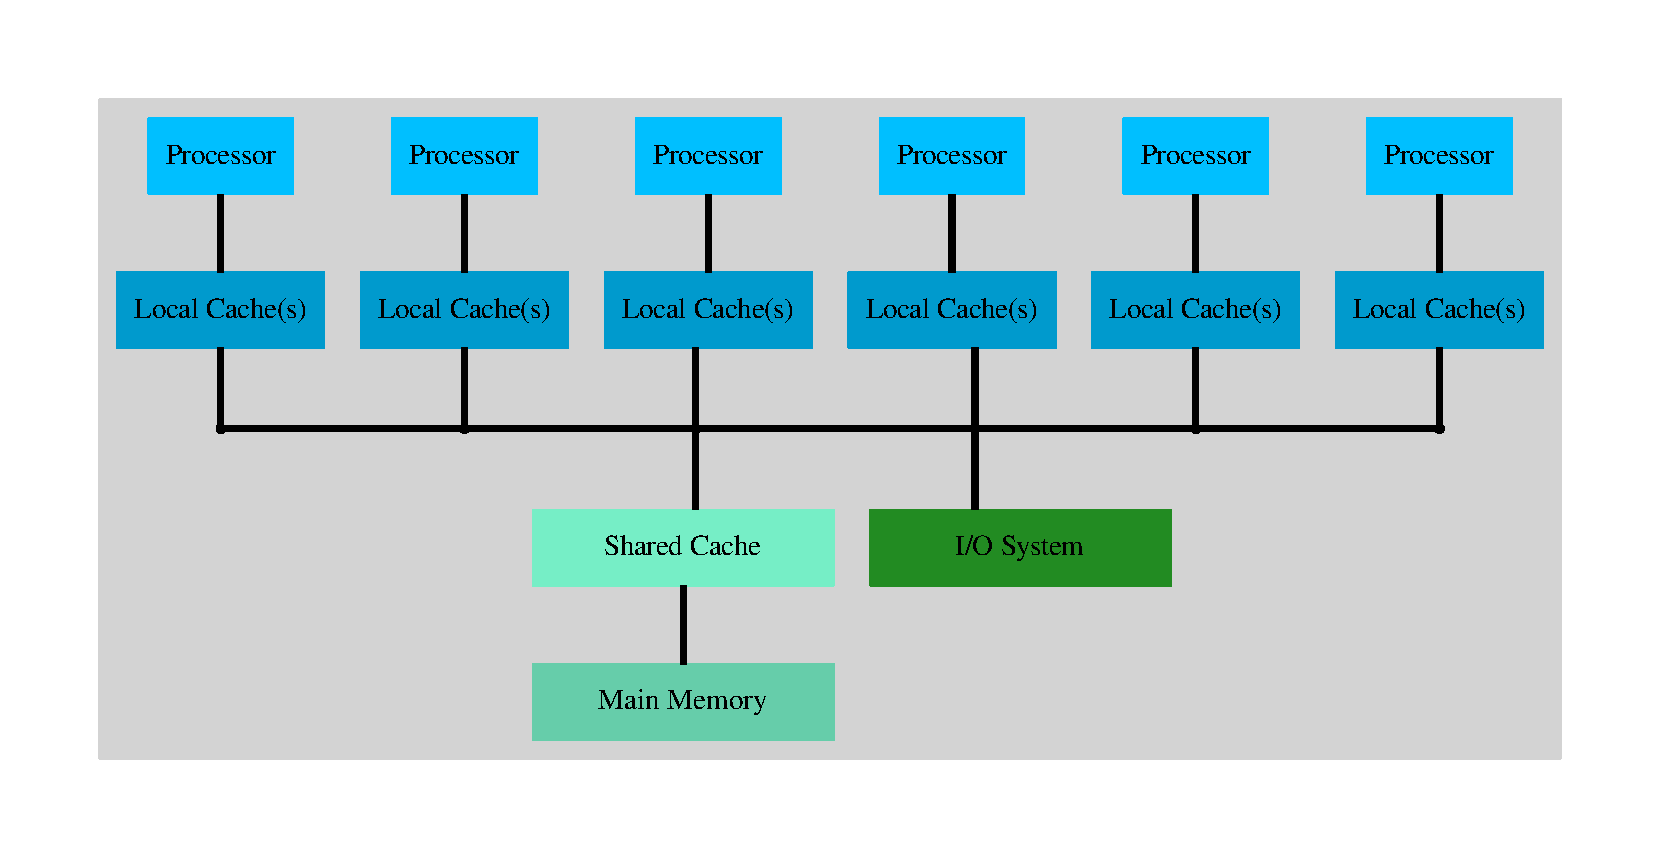
\includegraphics[width=0.75\textwidth]{figs/graphviz/smp.pdf}
    \caption{SMP System}\label{smp}
\end{figure}

\paragraph{A Distributed Shared Memory} sytem, also known as a Non-Uniform Memory Access
(NUMA) has mulitple memories that are distributed. In these systems, the memories are stilled
shared between processors, but access to different memories may take different amounts
of time. An interconnection network connects processors and memories together with one or
more processors per memory. Because memory access times can vary, software on NUMA systems
usually try to keep memory accesses local to a processor. However, NUMA systems can scale
much larger than SMP systems because contention to single memory does not necessarily increase
with an increasing number of processors. Figure \ref{distributed} illustrates what a typical
NUMA system might look like.

\begin{figure}[H]
    \centering
    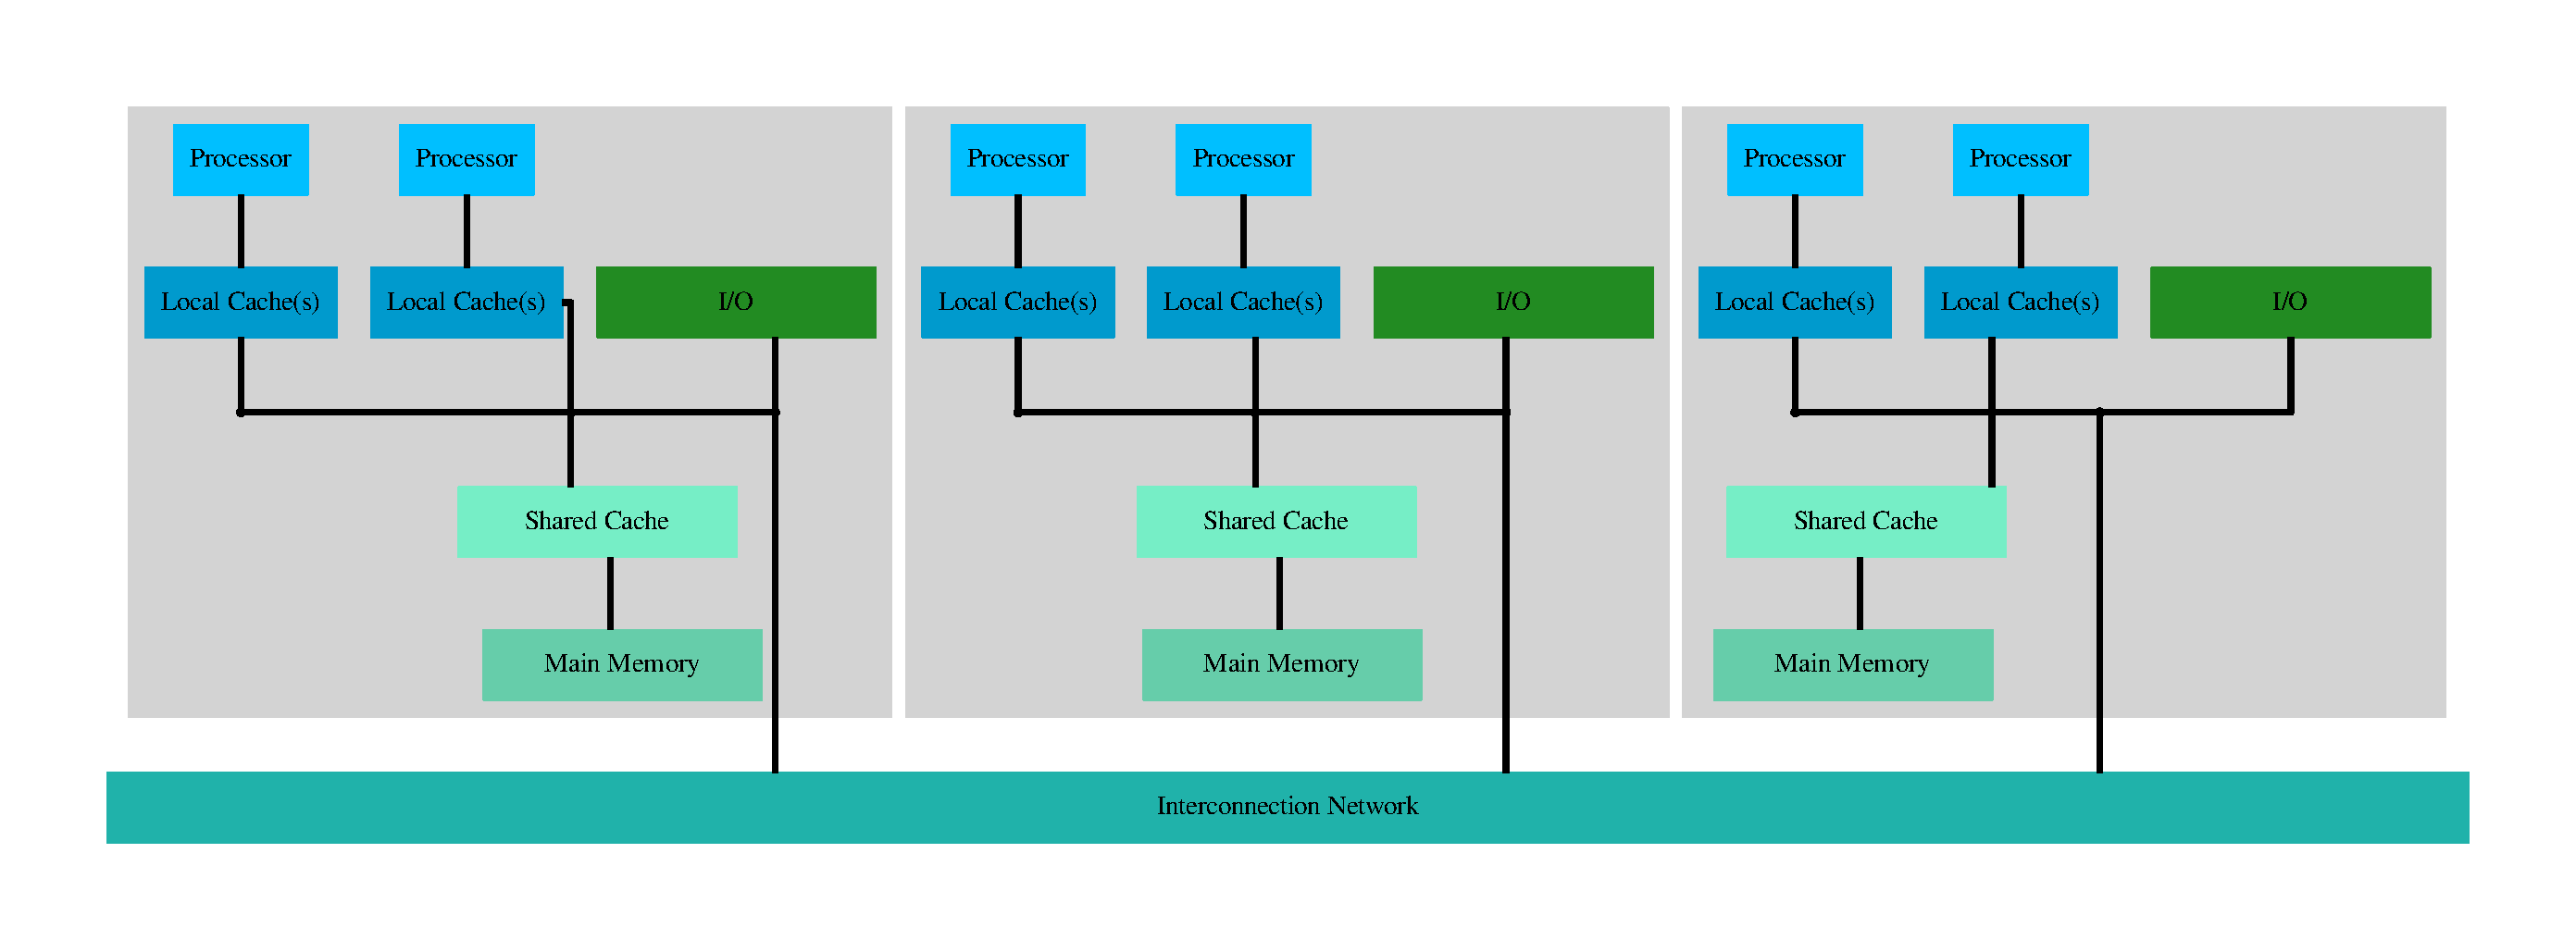
\includegraphics[width=\textwidth]{figs/graphviz/distributed.pdf}
    \caption{NUMA System}\label{distributed}
\end{figure}

\subsection{Clustered Systems}

\paragraph{A Beowulf Cluster} is a type of cluster which appears to the user as a single
machine. A single program is executed by all machines in the cluster and typically use
parallel communication software such as MPI or PVM.

\begin{figure}[H]
    \centering
    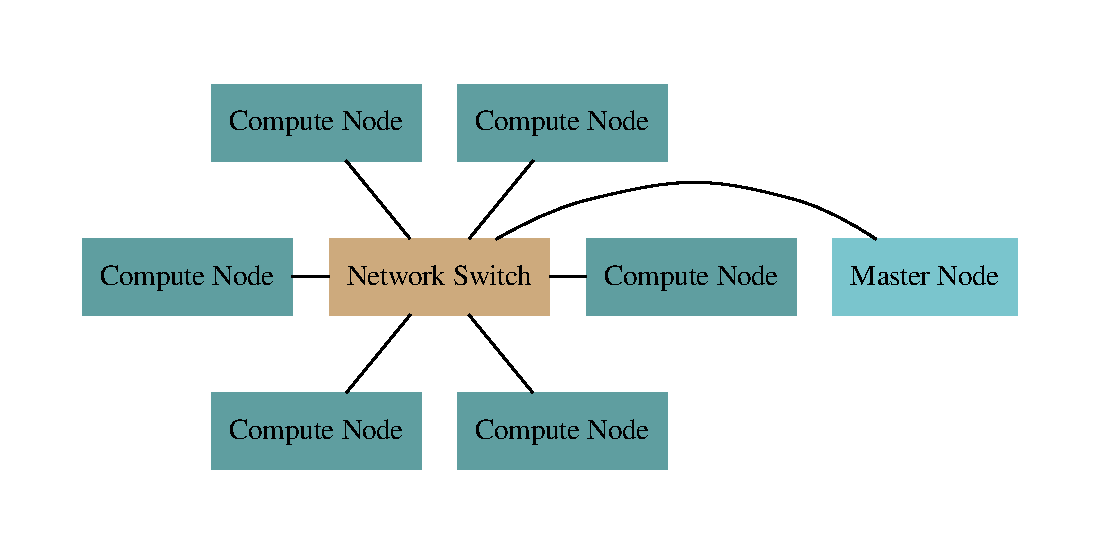
\includegraphics[width=0.6\textwidth]{figs/graphviz/beowulf.pdf}
    \caption{Beowulf Cluster}\label{beowulf}
\end{figure}

\section{Parallel Systems Communication}

Parallel applications are composed of multiple workers that operate independantly in parallel
and may have to exchange information. The workers in a parallel application can be a process,
thread, or any other type of execution context. Workers can communicate by either sending
explicit messages to each other by means of well defined message formats or by using shared
data structures that all workers can access. The former method is known as \emph{message passing}
and the latter method is known as \emph{shared memory}. Both communication models are
fundamentally different and both have strengths and weaknesses.

\subsection{Message Passing}

In a message passing system, workers are completely isolated in different address spaces
and communicate only through serialized messages. The formats of the messages must be
defined so that the message can be serialized and deserialized by the sender and the reciever,
respectively. Message passing can either be synchronous or asynchronous. With synchronous
message passing, the send/receive operations must be done in a specific order so that the
sender/receiver workers operate together in a synchronized fashion. The send operation at
the sender will block until the message is received at the reciever and the receive operation
at the receiver will block until the message is fully received. That means the every worker
must follow a predictable communication pattern. Workers cannot continue other operations
during communication operations and may slow down the whole system. On the other hand,
asynchronous communication allows workers to start send and recieve operations and immediately
continue without blocking. To allow this, intermediate queues must be used to hold pending
operations. The workers do not have to follow a predictable communication pattern in this
case because the messages will be queued and can be processed at any time and in any order.
The main advantage of message passing in general is that the number of workers can be scaled
very efficiently as long as the work is partitioned in the right way. The workers can execute
in address spaces on different machines and communicate over a local network. The biggest
disadvantage, however, is the high communication latency compared to computation speed.
Since workers run in different address spaces the messages must be copied or if the address
spaces exist on different machines, they must be propagated through the network. This makes
message passing especially hard for fine-grained parallel applications. An illustration of
simple message passing is shown in figure \ref{communication}.

\subsubsection{Message Passing Interface (MPI)}

MPI\cite{Forum:1994:MMI:898758} is an extensive message passing API specification for parallel
applications and supports both synchronous and asychronous forms of communication. MPI is just
a standard specification for developers and MPI users and many current implementations exist.
The most widely used implementations used in practice include MPICH and OpenMPI.

\subsection{Shared Memory}

The workers in a parallel application can also share a single address space and communicate
through shared data structures. The producer worker will insert data directly into the data
structure and the consumer worker will remove the data and use it. This takes much less time
to send data than message passing. However, access to the shared data structures must be
protected so that multiple workers do not simultaneously access the same data which could
cause unpredictable results. Access to the data is enforced using lock synchronization
mechanisms such as mutexes or semaphores. Shared memory data structures may suffer from
performance if lots of workers contend for the lock at the same time. For this reason, it
is very hard to scale systems that use only shared memory as a means of communication. An
illustration of a simple shared memory system is show in figure \ref{communication}.

\begin{figure}[H]
    \centering
    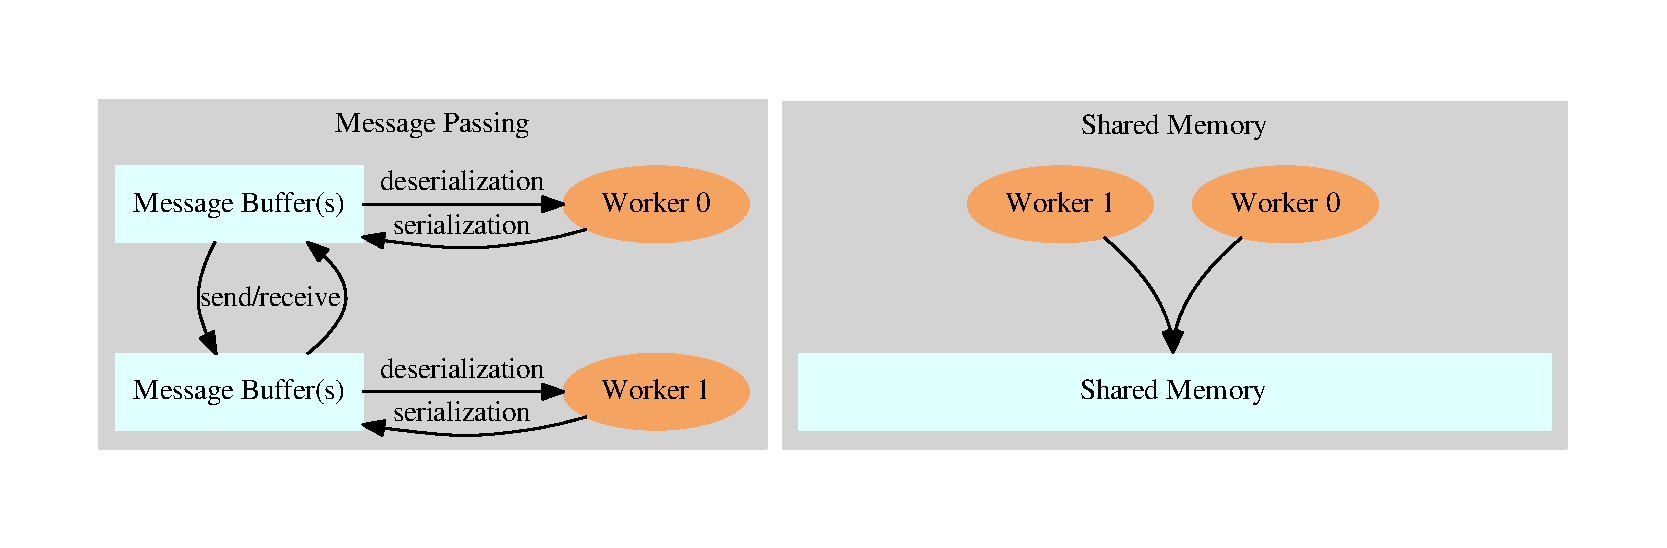
\includegraphics[width=\textwidth]{figs/graphviz/parallel_communication.pdf}
    \caption{Message Passing and Shared Memory Communication}\label{communication}
\end{figure}

\section{ARM big.LITTLE}

ARM big.LITTLE is a computer architecture design which uses a combination of powerful
processor cores that use a lot of power (big) with slower, more power-efficient processor
cores (LITTLE). The purpose of this design is to allow good performance when the system load
is heavy by running tasks on the big cores while also allowing power savings when the system
load is low by running tasks on the LITTLE cores. The operating system CPU scheduler can
make use of the big.LITTLE architecture in multiple ways by using different task allocation
and switching policies. The three main methods that are currently being used in practice
are cluster switching, CPU migration, and heterogeneous multi-processing. The remainder of
this section describes the three methods in more detail.

\subsection{Cluster Switching}

With cluster switching, the LITTLE cores and big cores are grouped into \emph{clusters} with
the big cores in one cluster and the LITTLE cores in another cluster. At any point in time,
the OS scheduler will only schedule tasks to cores within a single cluster. When the system
gains enough load so that a big core is needed, then the OS scheduler must switch to the big
cluster and only use the big cores. This is the simplest method but can still waist a lot
power by unnecessarily switching to the big cluster. Furthermore, only half of the cores are
available at time which prohibits the use of full computational capacity. A diagram that
illustrates cluster migration is shown in figure \ref{cluster_switching}.

\begin{figure}[H]
    \centering
    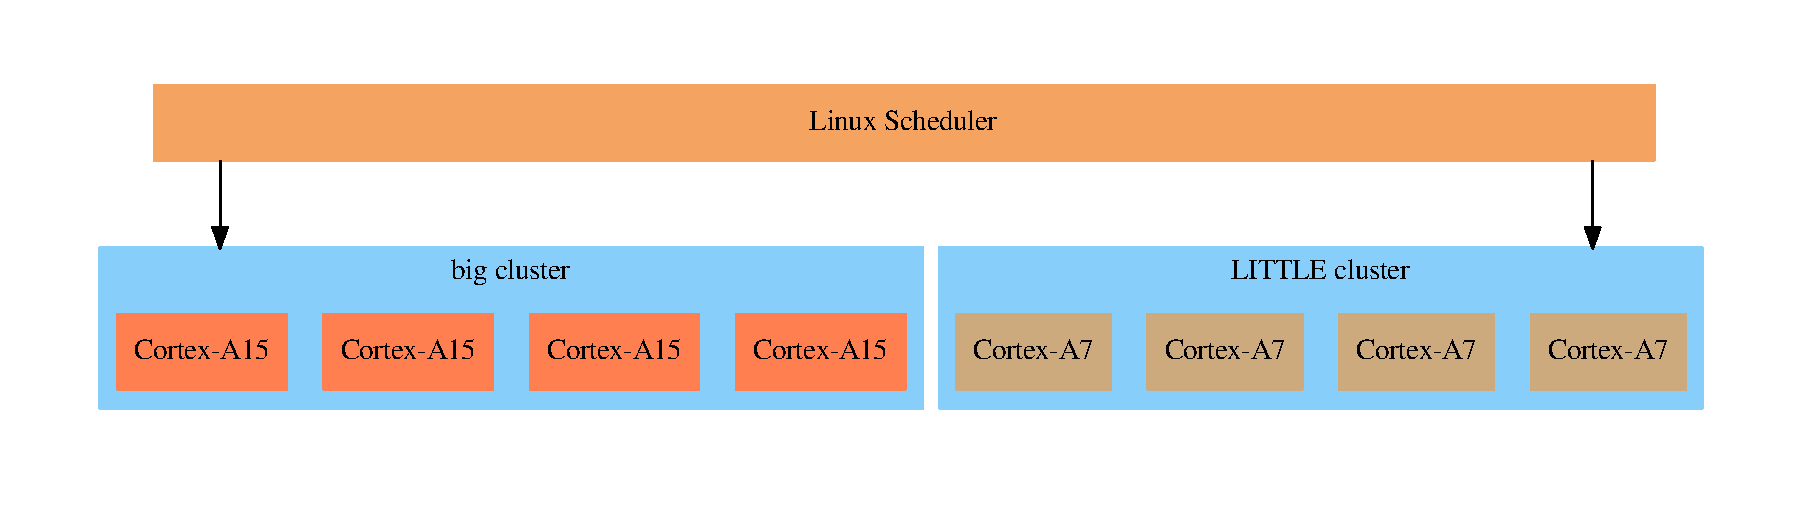
\includegraphics[width=\textwidth]{figs/graphviz/cluster_switching.pdf}
    \caption{Cluster Switching}\label{cluster_switching}
\end{figure}

\subsection{CPU Migration}

CPU migration is the next step up from cluster switching. With CPU migration, each big
core is paired with a LITTLE core and the OS treats them as a single virtual core. At any
point in time, the OS scheduler will only schedule tasks to only one of the physical cores
within each virtual core. The advantage of this approach over cluster switching is that if
the load on the system is only large enough so that a single big core is needed then power
isn't waisted because only a single big core will be switched on. Like cluster switching
though, only half the of CPU cores are available at a time which still prohibits full
computational capacity of the system. A diagram that illustrates cpu migration is shown in
figure \ref{cpu_migration}.

\begin{figure}[H]
    \centering
    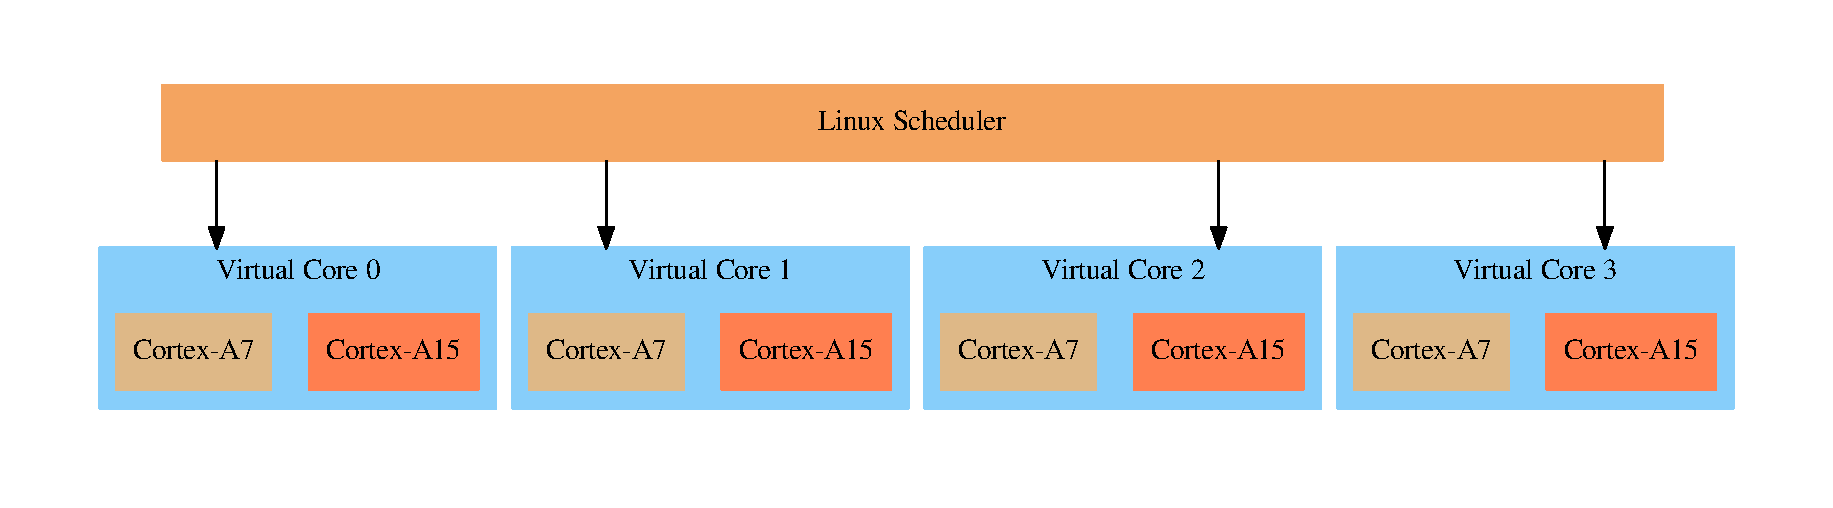
\includegraphics[width=\textwidth]{figs/graphviz/in_kernel_switcher.pdf}
    \caption{CPU Migration}\label{cpu_migration}
\end{figure}

\subsection{Heterogeneous Multi-Processing (HMP)}

Heterogeneous Multi-Processing or Global Task Scheduling (GTS) allows simultaneously
scheduling to all CPU cores at the same time. The tasks that have a higher priority or
require more processing power will be scheduled to the big cores whereas the tasks with
low priority that don't require much processing power, such as background tasks can be
scheduled to the LITTLE cores. This is the most complex approach and is hard to implement
because the OS scheduler must not treat all cores the same. Policies to allocate tasks
must be implemented in the proper manner as well as policies for migration of task to and
from the big cores and LITTLE cores. Much research is still in progress to determine the
right policies. A diagram that illustrates HMP is shown in figure \ref{global_task_scheduling}.

\begin{figure}[H]
    \centering
    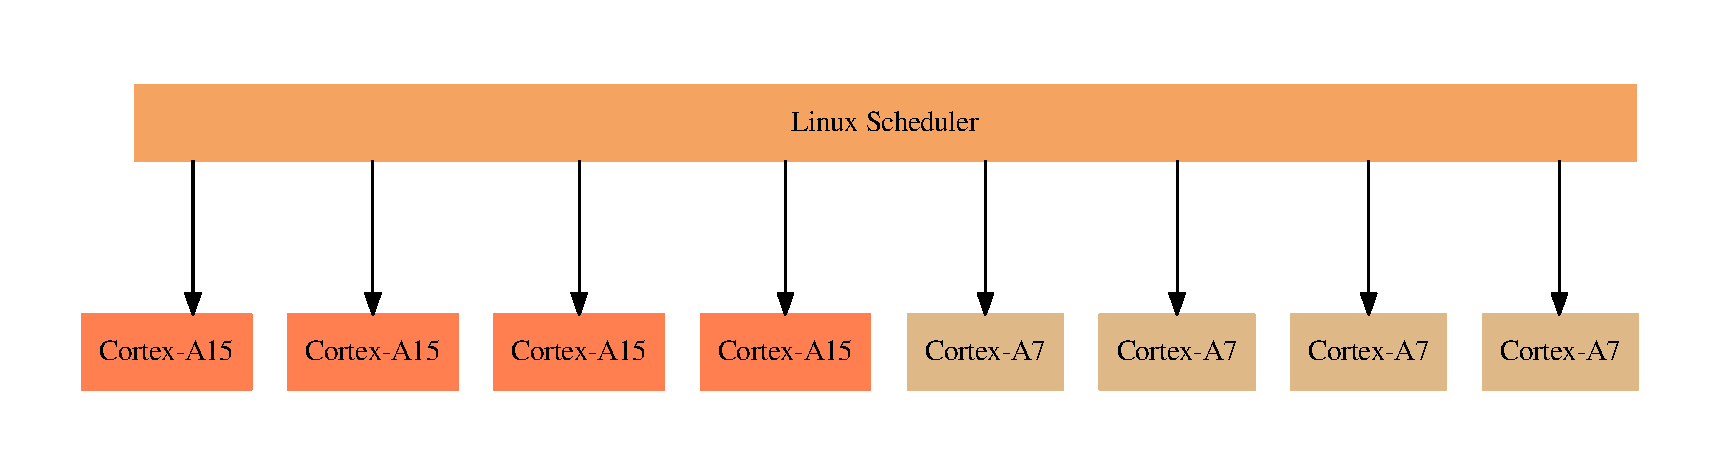
\includegraphics[width=\textwidth]{figs/graphviz/global_task_scheduling.pdf}
    \caption{Heterogeneous Multi-Processing}\label{global_task_scheduling}
\end{figure}



\chapter{Related Work}\label{related_work}

This chapter give an overview of some of the most popular Time Warp systems. For each system,
the design will be described at a high level. The the data structures and algorithms used
will be described further as well as the strengths and weaknesses.

\section{Georgia Tech Time Warp (GTW)}

Georgia Tech Time Warp is a general purpose Time Warp Simulator designed specifically for
shared memory multiprocessors. Although GTW is not used any more, it's design has influenced
the design of other simulators that are used widely in practice. GTW simulation models run
in a single processes, multi-threaded environment and uses only shared memory to communicate
between threads that are bound to single processor. The LP's for all models are statically
allocated to a single thread so that events for the LP's are processed only on a single
processor.

The pending event set is distributed among threads with each having its own data structures.
Since the threads can only run on a single processor, the data structures are owned by that
processor. The pending event set for each processor consists of three main data structures
listed below\cite{das-94}:

\begin{enumerate}
    \item The \emph{Message Queue} is a linked list that contains positive messages that
        are destined for the LP's mapped to the owning processor. Access to the message
        queue must be synchronized because it can be accessed by tasks running on any processor.
    \item The \emph{Cancel Queue} is a linked list that serves exactly the same purpose as
        the message queue except that it containes only negative messages(anti-messages).
        Access to this queue must also be synchronized.
    \item The \emph{Event Queue} is used to hold unprocessed and processed events and is
        directlyused to schedule events to be processed. The event queue is actually made
        up of different data structures, one for processed events and one for unprocessed
        events. The processed events are contained within a doubly linked list and the
        unprocessed events are contained within a priority queue which can be configured to
        be either a calendar queue or a skew heap depending on a user configuration.
\end{enumerate}

\noindent
When messages are sent between LP's, they are inserted directly in the message queue or
the cancel queue depending on whether they are positive or negative. Each thread first moves
messages from the message queue to the event queue and processes any rollbacks. Then, the
messages from the cancel queue are removed and cancellations and any more rollbacks are
processed. The smallest event from the event queue is then processed and added to the
processed event list. This procedure is repeated over over and over again by all processors.
Psuedocode for the main event processing loop in GTW is show in figure \ref{gtw_processing}.

\begin{algorithm}
\DontPrintSemicolon
\SetAlgoVlined
    \While{eventQ is not empty} {
        move messages from MsgQ to EvQ and process any rollbacks\;
        remove anti-messages from CanQ, process annihilations and rollbacks\;
        remove smallest timestamped event E from EvQ\;
        processe event E\;
    }
\caption{GTW Main Event Processing Loop\cite{das-94}\cite{fujimoto-94}\label{gtw_processing}}
\end{algorithm}

\noindent
To avoid accessing the message queues and cancel queues too often, which is a contention point,
GTW also supports batch processing. With batch processing, multiple events will be processed
at a time without processing any rollbacks or cancellations.

The partitioning of the LP's among processors must be done in the simulation model during
initialization. That means that the model developer must understand some the features of
the underlying architecture such as the number of processors, to effectively partition the
LP's. Furthermore, the initial partitioning of the LP's is hard to change during the course
of the simulation because there are no seperate input queues but rather a single message
queue to hold all unprocessed events for each processor.

%% The states of the LP's can be save using the traditional copy-state saving or incremental
%% state saving. The simulation model must choose which state variables need to be automatically
%% saved after every processed event and which state variables need to be incrementally saved.
%% The state variables must then be registered with the simulation kernel so that they can
%% saved when needed and restored when a rollback occurs. The state saving mechanisms provided
%% allow the simulation model developer some flexability to optimize the simulation model based
%% on how often the state variables are modified. The seldom modified variables can be
%% incrementally saved and the often modified variables can always be saved. However, it also
%% forces the simulation model developer to understand time warp and how the underlying state
%% saving mechanisms work.

%% GTW does not use conventional fossil collection. Instead, the events are placed into a
%% per thread free list after they are processed. Events can then be allocated from the free
%% list as long as the first event in the list has a timestamp less than the GVT. If the first
%% event is not less than the GVT then the current event being processed is aborted and fossil
%% collection is initiated. This mechanism called "on-the-fly" fossil collection. One benefit
%% to on-the-fly fossil collection is that it provides a mechanism to prevent some LP's from
%% processing events too far in the future. However, on-the-fly fossil can cause unstable
%% behavior. As rollbacks occur, the free lists becomes unordered and the first event in the
%% list may not have a timestamp less than the GVT even if another event in the list does.
%% If a processor tends to have LP's that rollback more often, then a lot of events can be
%% unnecessarily aborted because it is becomes more unordered relative to other free lists.
%% Searching the free-list will also not help because it will take more time to search longer
%% lists which will cause behavior to still  depend on rollback behavior. The only way to fix
%% the problem with imbalanced event processing is to allocate more memory per processor.

%% GTW versions only exist for SparcStation and SGI PowerChallenge architectures.

\section{Clustered Time Warp (CTW)}

Clustered Time Warp\cite{avril-95} (CTW) uses a hybrid approach by processing events within
a \emph{cluster} of LP's sequentially and using the Time Warp mechanism between the clusters.
This design was chosen because it works well for digital logic simulation which tend to have
localized computation within a group of LP's. Furthermore, digital logic simulation tends to
have low computational granularity and lot's of LP's which can lead to a lot of rollbacks
and a large memory footprint in a traditional Time Warp simulator. CTW is implemented for
shared memory multiprocessors but only uses shared memory for use with a message passing
system. No other shared memory algorithms are used.

Each cluster has a timezone table, an output queue, and a set of LP's which each have an
input queue and a state queue. The timezones in the timezone table are divided by timestamps
of the events received from LP's on different clusters. Whenever an event is received from
a remote cluster, a new timezone is added. Only a single output queue is needed per cluster
because anti-messages can only be sent between clusters and not between LP's on the same
cluster.

When a straggler event arrives at a cluster, all of the LP's that have processed events that
are greater than the timestamp of the straggler will be rolled back. This rollback scheme is
called \emph{clustered rollback}. The alternative to clustered rollback is \emph{local
rollback}. In a local rollback scheme the straggler event would be inserted into the receiver
LP's input queue and the LP will roll back when it is detected. Although clustered rollbacks
may cause some LP's to be rolled back unnecessarily leading to slower compuation, the
approach was chosen for CTW because processed events will not have to be saved which
requires less memory.

CTW uses a form of infrequent state savings with the timezone table used to determine the
frequency. When an event is about to processed for an LP, the timezone of the last processed
event is looked up and if event that is about to be processed is in a different timezone then
the state is saved. This approach in which all LP's save their state every time an event is
processed in a new timezone regardless of whether it receives an event from a remote cluster
is called \emph{local checkpointing}. This method reduces the state saving frequency more
than a \emph{clustered checkpointing} approach in which only the LP that receives an event
from a remote cluster saves its state. The local checkpointing approach was chosen for CTW
because a larger state saving frequency can increase rollback computation and it can even
lead to more memory consumption because more events must be saved for coast forwarding
during state restoration.

\section{Rensselaer's Optimistic Simulation System (ROSS)}

ROSS\cite{carothers-00} is a general purpose simulator that is capable of running both
conservatively and optimistically synchronized parallel simulations as well as sequential
simulations. It is most often used for optimistic parallel simulations which is achieved
with the time warp mechanism. ROSS started as a reimplementation of GTW and is still
modeled after it but has some enhancesments. The same basic event scheduling mechanism is
used but ROSS supports different priority queue implementations and different algorithms
are used for fossil collection, state saving, and gvt calculation. In addition, ROSS uses
processes instead of threads and uses message passing with MPI instead of shared memory
for communication among the processes.

Just as in GTW, ROSS maps every LP to a process and each process contains its own pending
event set structures. No locks are needed explicity within each process because there are
no shared data structures among processes. The data structures are very similar to those
used in GTW but have a different naming convention. The main data structures in ROSS are:

\begin{enumerate}
    \item The \emph{Event Queue} is analogous to the message queue in GTW. It contains the
        positive events for all LP's in the corresponding process. In addition, an event
        queue is used to hold all remote events regardless of whether it is positive or
        negative. The event queue is implemented as a linked list.
    \item The \emph{Cancel Queue} is a linked list which is used to hold negative events
        for all LP's for the corresponding process. The cancel queue is used in the exact
        same way as GTW except that no locks are necessary.
    \item The \emph{Priority Queue} is analogous to the event queue in GTW and contains
        events in timestamp order. ROSS also allows the priority queue to be implemented
        as a calendar queue, heap, splay tree, or avl tree depending on user configuration.
\end{enumerate}

\noindent


%% ROSS does not save any of the LP's state, but instead uses reverse computation
%% \cite{carothers-99a} to restore states. With reverse computation, a sequence of bits is
%% saved for each event which describes the path of execution (control state). By knowing the
%% path of execution for each event, it is possible to know exactly what state variables were
%% modified and how. This method works great for some models but relies on two main properties.
%% The first property that the models should have is that the reverse computation should not
%% rely on previous values of the state variables. The second property that the  models should
%% have is simple forward computation that contains very few branches. More complex code
%% will lead to a larger control state which can end up being as large or larger than the data
%% state of the LP's.

%% Because of the limitations of on-the-fly fossil collection, ROSS does not use it and instead
%% uses conventional fossil collection triggered by a GVT change. To make fossil collection
%% more efficient, LP's within are further divided into units called Kernel Processes (KPs).
%% The LP's within each KP are then fossil collected together. Furthermore, because the
%% processed events within a KP are grouped together, the KP's must also be rolled back as a
%% single unit just like clustered rollback in Clustered Time Warp.

\section{\textsc{warped}}

\textsc{warped} is the predecessor of \textsc{warped2}. The complexity of \textsc{warped}
became unmaintainable over the years which eventually led to its demise and rewrite.
\textsc{warped}, from its beginnings, has always followed a modular design to allow maximum
flexability for new optimization.

The famous computer scientist David Wheeler used to say "All problems in computer science
can be solved by another level of indirection."

Kevlin Hennley's corallary to goes "...except for the problem of too many layers of
indirection."

The original \textsc{warped} was written for 

\section{Others}

\subsection{The ROme OpTimistic Simulator (ROOT-Sim)}

ROOT-Sim is another general purpose Time Warp Simulator that uses message passing via MPI
\cite{pellegrini-11}. Like \textsc{warped}, ROOT-Sim is a more classic Time Warp
implementation with each LP having their own input queues, and output queues. What sets
ROOT-Sim apart from other time warp simulators is the internal instrumentation tool, Dynamic
Memory Logger and Restorer (DyMeLoR) that can optimize memory usage. DyMeLoR can determine
whether the simulation models are better fit for copy-state saving or incremental state
saving and transparently switch between them during runtime. Another service that ROOT-Sim
offers is the Committed and Consistent Global Snapshot (CCGS). After each GVT calculation,
ROOT-Sim transparently rebuilds a global snapshot of all LP states. Each LP can access its
portion of the global snapshot on every GVT calculation. With this service, a simulation
model can implement any custom global snapshot algorithm.

\subsection{ROSS-MT}

ROSS-MT\cite{jagtap-12} is a multi-threaded version of ROSS which is optimized to use shared
memory to communicate among threads. The use of message passing with MPI was completely
removed and all events are sent by direct insertion into the event queues. To reduce the
added contention on the event queues, they are further divided by possible senders. ROSS-MT
also optimizes the free memory lists so that they are more NUMA aware. Instead of allocating
memory from the receiver processors free list, it is allocated from the senders free list.
Furthermore, a LIFO approach is taken to improve cache reuse.



\chapter{The \textsc{warped2} Simulation Kernel}\label{warped2_overview}

This chapter describes the software architecture of the \textsc{warped2} simulation kernel.
The main compenents are described. The modeling API is also described and an example model
is shown to illustrate the API.

\section{The Software Architecture of \textsc{warped2}}

The \textsc{warped2} simulation kernel uses a modular design to make it configurable,
extendable, and maintainable.

\subsection{Event Dispatcher}

The event dispatcher is at the center of everything and determines how the simulation will
be progressed. Warped2 currently supports the event dispatcher to be configured for either
sequential simulation or time warp simulation. The sequential event dispatcher just contains
a single list of all events because only a single event is processed at a time. The time warp
event dispatcher has more complex data structures and multiple components. In either case,
the event dispatcher calls methods that are defined by the LP. Since a sequential simulation
doesn't really have any real complexity only the time warp event dispatcher will be discussed
any further. The time warp components are illustrated in figure \ref{warped2_architecture}.

\begin{figure}[H]
    \centering
    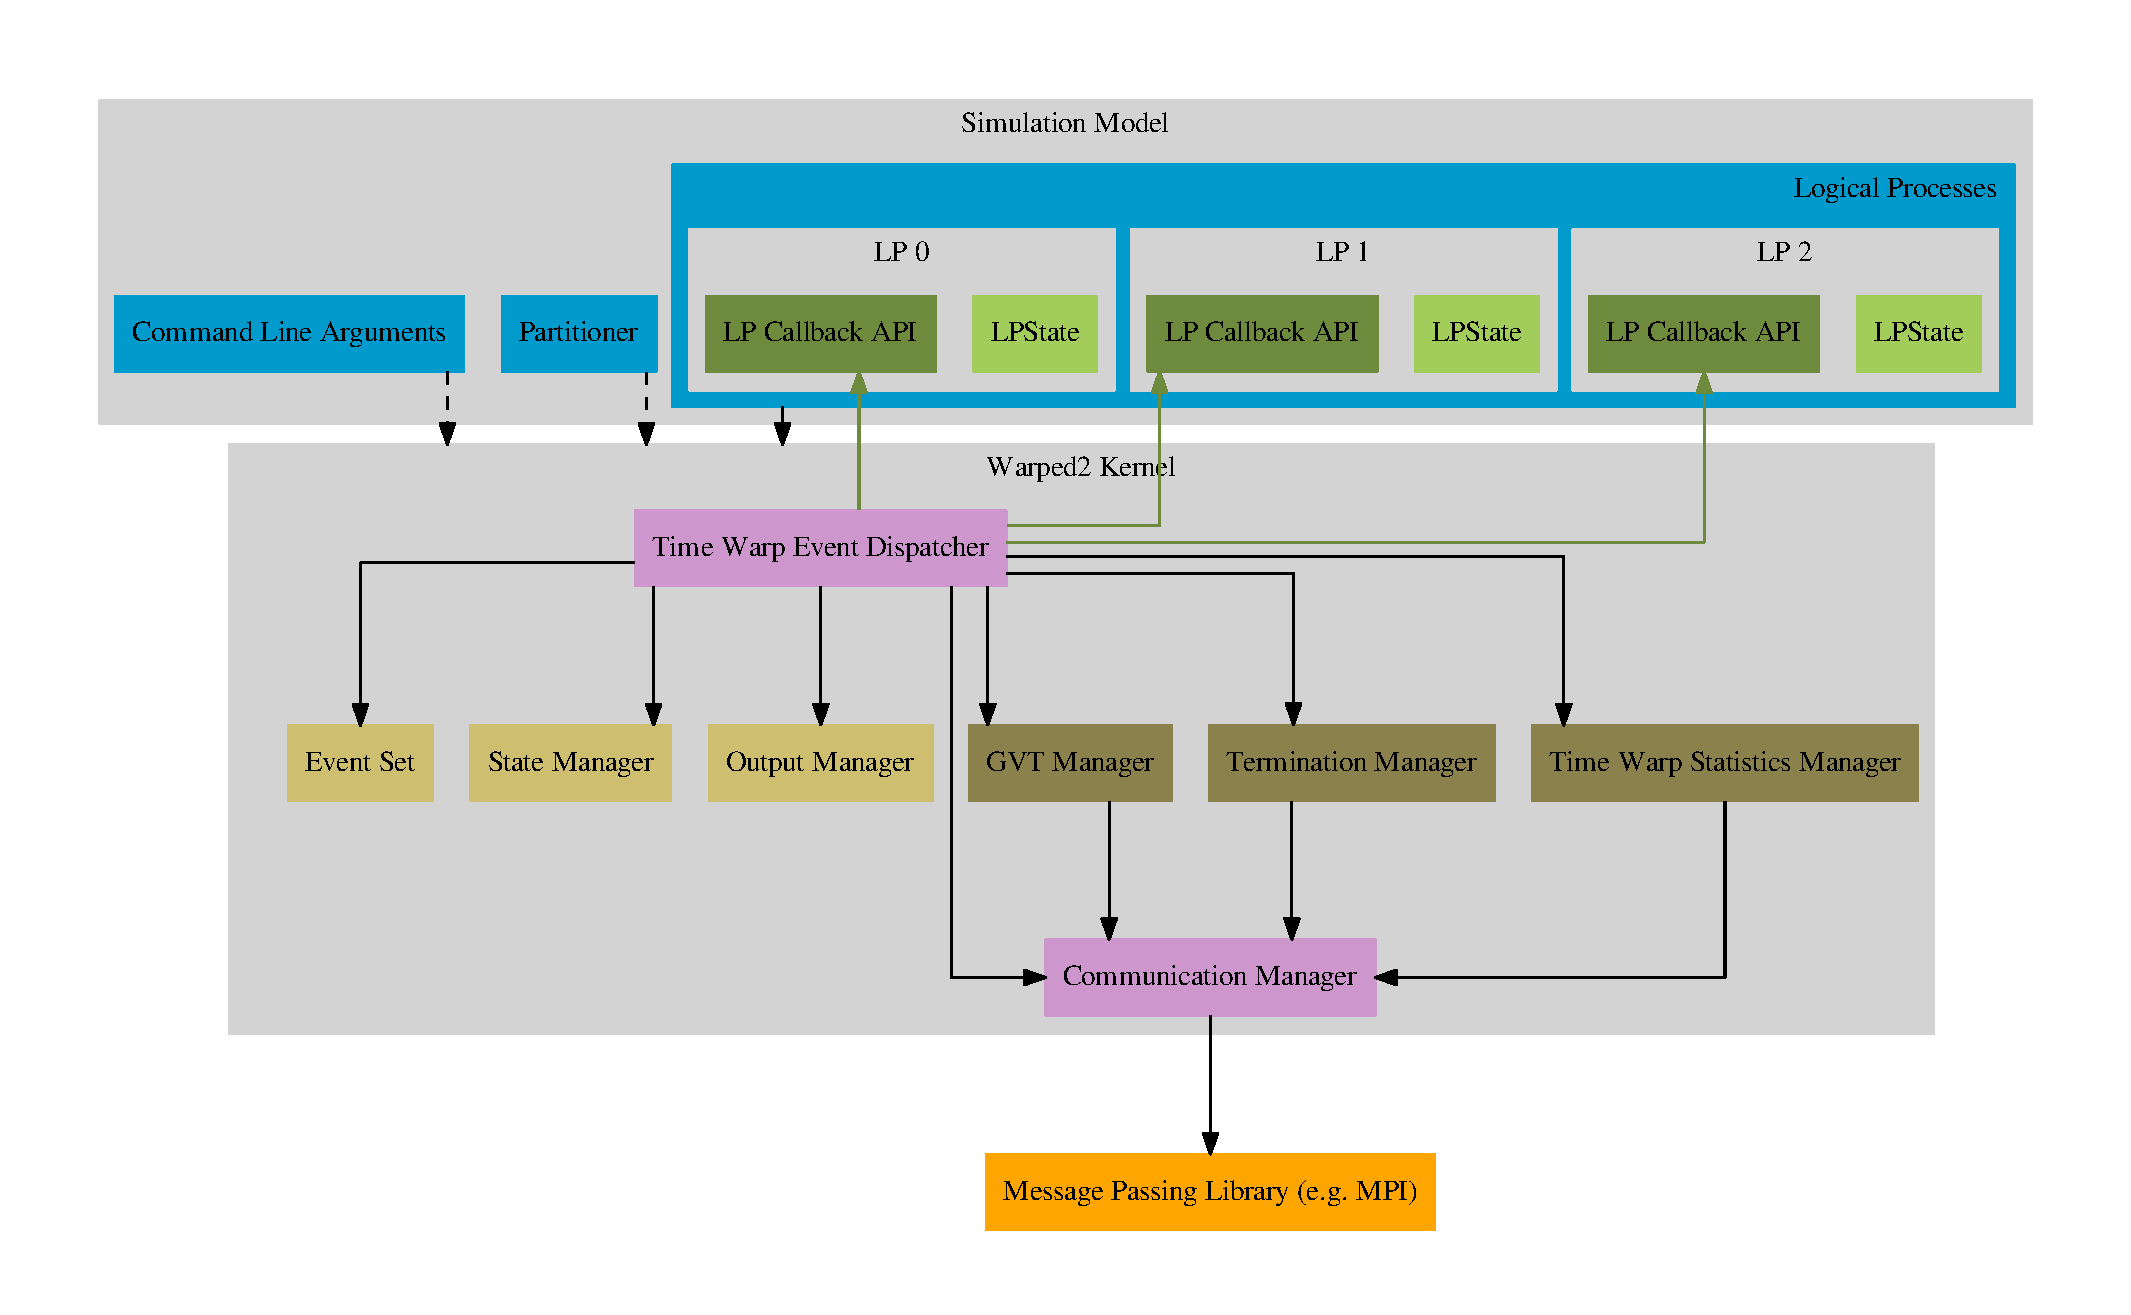
\includegraphics[width=\textwidth]{figs/graphviz/warped2_overview.pdf}
    \caption{Time Warp Components in \textsc{warped2}}\label{warped2_architecture}
\end{figure}

\noindent
Each process has its own time warp components that exist in only their own address space.
The time warp components can be categorized as either a local time warp component or a global
time warp component. The local time warp components are concerned only with the local control
mechanism of the individual LP's such as rollbacks and fossil collection whereas the global
time warp components are concerned with the global control mechanisms such as GVT, termination
detection and statistics counting.

\subsection{Local Time Warp Components}

\paragraph{The Event Set} contains the data structures for all of the unprocessed and
processed events for the LPs that are local to the process. This is where the events are
scheduled for processing. It provides methods for getting the next event, rolling back an
LPs input queue, and fossil collecting the processed events for an LP.

\paragraph{The Output Manager} contains all of the output queues and implements a cancellation
technique. It provides methods for adding an event to an LPs output queue, rollback back an
LPs output queue, and fossil collecting old output events. Currently, \textsc{warped2} only
supports aggressive cancellation.

\paragraph{The State Manager} contains all of the state queues and implements a technique
for saving and restoring states for the LPs. It provides methods for saving the state of an
LP, restoring the state of an LP, and fossil collecting old states. Currently, \textsc{warped2}
only supports periodic state saving.

\subsection{Global Time Warp Components}

\paragraph{The GVT Manager} implements an algorithm for determining the Global Virtual Time
of the simulation. A more detailed description of the GVT algorithm used in \textsc{warped2}
is given in chapter \ref{gvt_termination}.

\paragraph{The Termination Manager} impements an algorithm for determining when all processes
become inactive and initiates termination when that occurs. A more detailed description of
the termination algorithm used in \textsc{warped2} is given in chapter \ref{gvt_termination}.

\paragraph{The Time Warp Statistics Manager} keeps track of all local statistics counts and
provides methods to do global reductions on the statistics.

\subsection{Communication Manager}

The communication manager provides an interface between the underlying message passing library
and the \textsc{warped2} simulation kernel. Any interprocess communication must go through the
communication manager whether the communication processes are on the same machine or different
machines.

\section{The Modeling API of \textsc{warped2}}

The modeling interface of warped2 is a set of abstract base classes that contain methods
that must be implemented in a derived class. The base classes may also contain methods and
data members that are available to use by the derived classes. The three main base class
types that must be implemented are LogicalProcess, LPState, and Event. Optionally, the user
may create a custom partitioner from the Partitoner base class. In the remainder of this
section, each class is described in more detail and sample implementations are shown for each.

\subsection{The LPState Structure}

The state of the LP's must be define with the \textsc{warped\_define\_lp\_state\_struct}
macro. This is used to ensure that the warped2 kernel can save a copy of the state and
restore the state from a pointer to the LogicalProcess base class. An intermediate template
class is defined which defines the necessary methods to make a copy of the state and to
restore the state so that the user does need to explicitly define them. However, if the
state contains complex data structures that contains pointers then the default copy
constructor and default copy assignment operator will only perform shallow copies. In this
case the user must implement a custom copy constructor or a custom copy assignment operator
or both. The copy constructor will define the behavior for saving the state whereas the
copy assignent operator will define the behavior for restoring the state. Note that the
copy assignment operator will most likely not be needed since a shallow copy will usually
suffice. A simple example of a LP state that contains just message counts is shown
below in listing \ref{example_state}.

\begin{lstlisting}[caption=Example \textsc{warped2} State Definition, label=example_state, float]
WARPED_DEFINE_LP_STATE_STRUCT(ExampleState) {
    unsigned int messages_received_;
    ...
};
\end{lstlisting}

\subsection{The Event Class}

The event base class is used as the basis for creating model specific events. The user must
implement at least two function: \texttt{receiverName()} and \texttt{timestamp()} so that
the name of the receiver and receive time, respectively, can be obtained for each instance
of an event. The user must also register all member variables with the serialization API so
that a storage order can be defined for events that are sent and received over a network.
To do this, the WARPED\_REGISTER\_SERIALIZABLE\_MEMBERS macro is provided. All member
variable must be passed to this macro as well as
\texttt{cereal::base\_class<warped::Event>(this)} to ensure that all members that are
inherited are also serialized serialized. The order that the members are listed is completely
arbitrary and does not matter. In addition, the derived event type must be registered using
the WARPED\_REGISTER\_POLYMORPHIC\_SERIALIZABLE\_CLASS macro. A basic example of an event
implementation is shown below in listing \ref{event_example}.

\begin{lstlisting}[caption=Sample \textsc{warped2} Event Definition, label=event_example, float]
class ExampleEvent : public warped::Event {
public:

    ...

    const std::string& receiverName() const { return receiver_name_; }
    unsigned int timestamp() const { return time_stamp_; }

    ...

    std::string receiver_name_;
    unsigned int timestamp_;

    ...

    WARPED_REGISTER_SERIALIZABLE_MEMBERS(cereal::base_class<warped::Event>(this),
                                         receiver_name_, timestamp_, ...)
};
WARPED_REGISTER_POLYMORPHIC_SERIALIZABLE_CLASS(ExampleEvent)
\end{lstlisting}

\subsection{The LogicalProcess class}

The most important class definition in the simulation model is the LogicalProcess class.
The implementation of the LogicalProcess class defines the callback functions that the
warped2 kernel calls and thus defines the behavior of the simulation. The user must include
a single LPState implementation as well three method implementations:

\begin{enumerate}
    \item The \texttt{initializeLP} method is called to perform any initializations that must
        be done prior to the start of the simulation and must return a set of initial events.
    \item The \texttt{receiveEvent} method is called to perform some computation based on
        the event that is passed. The implementation of this method interprets the event,
        updates the state of the LP and returns a set of new events with future timestamps.
    \item The \texttt{getState} method provides a way for the warped2 kernel to get the current
        state of the LP.
\end{enumerate}

It is necessary that at least one LP has an initial event that is returned by
initializeLP, otherwise no events can be received and simulation will terminate immediately.
Also note that the it will be called once for \emph{every} LP instance so it is possible that
initial events are returned only in some cases. An example of a LogicalProcess implementation
is shown below in listing \ref{lp_example}.

\begin{lstlisting}[caption=Example \textsc{warped2} LogicalProcess Definition, label=lp_example, float]
class ExampleLP : public warped::LogicalProcess {
public:

    ...

    warped::LPState& getState() { return this->state_; }

    std::vector<std::shared_ptr<warped::Event> > initializeLP() override {
        this->registerRNG(this->rng_);
        std::vector<std::shared_ptr<warped::Event> > events;
        ...
        return events;
    }

    std::vector<std::shared_ptr<warped::Event>> receiveEvent(const warped::Event& event) {
        ++this->state_.messages_received_;
        std::vector<std::shared_ptr<warped::Event> > response_events;
        ...
        return response_events;
    }

    ExampleState state_;
};
\end{lstlisting}

\subsection{The Partitioner class}\label{partitioner}

The warped2 kernel already provides a round-robin partitioner and a profile-guided partitioner
but the user can define their own partitioner that is customized for a specific model.
The user must derive from the Partitioner base class and implement just a single method
which takes a vector of all LP'ss and the number of partitions desired and returns a vector
of vectors of LP's. In general, the partitioner should work for any number of partitioners
and not impose any constraints because the partition method is called back from the kernel.
A simplified version of the kernel's round-robin partitioner is shown in listing
\ref{partitioner_example}. Note that a model would never have to implement such a general
partitioner but is showed just as a simple example.

\begin{lstlisting}[caption=Example \textsc{warped2} Partitioner Definition, label=partitioner_example, float]
class ExamplePartitioner : public Partitioner {
    std::vector<std::vector<LogicalProcess*>>
    partition(const std::vector<LogicalProcess*>& lps, const unsigned int num_partitions) {
        std::vector<std::vector<LogicalProcess*>> parts;
        ...
        return parts;
    }
};
\end{lstlisting}

\subsection{Random Number Generation}

If the simulation model uses random number generators, they must all be registered with the
warped2 kernel. This is necessary so that the state of the random number generator can be
saved and restored in case of rollbacks. The random number generators can be any type as
long as they implement the \texttt{<< operator} and \texttt{>> operator} to allow the kernel
to save and restore the internal state of the random number generator. To register the
random number generator, the registerRNG template function must be used which is a member
of the LogicalProcess class. All LP's must have separate random number generators and must
be registered in the initializeLP callback function as shown in listing \ref{lp_example}.

\subsection{Command Line Arguments and the Kernel Entry Point}

Once all the necessary structures and classes have been defined, the model's main function
must be implementd which is where all calls into the kernel are made. First, the model
specific command line arguments must be registered with the kernel. This must be done first
so that it can be passed to the constructor of a \texttt{Simulation} instance. Then all of
the LP's and optionally a partitioner must be instantiated and passed to the kernel through
the \texttt{simulate} method of \texttt{Simulation} object. Two versions of the simulate
methods are available, one for a model with a custom partitioner and one without as listed below:

\begin{enumerate}
    \item \begin{verbatim} void simulate(const std::vector<LogicalProcess*>& lps); \end{verbatim}
    \item \begin{verbatim} void simulate(const std::vector<LogicalProcess*>& lps,
                std::unique_ptr<Partitioner> partitioner); \end{verbatim}
\end{enumerate}

\noindent
A sample implementation of a models main function is shown in listing \ref{main_sample}.

\begin{lstlisting}[caption=Sample \textsc{warped2} Main Definition, label=main_sample, float]
int main(int argc, const char **argv) {
    unsigned int num_lps = 10000;

    TCLAP::ValueArg<unsigned int> num_lps_arg("o", "lp-count", "Number of lp's", false,
                                              num_lps, "unsigned int");
    std::vector<TCLAP::Arg*> cmd_line_args = {  &num_lps_arg };
    warped::Simulation simulation {"Sample Simulation", argc, argv, cmd_line_args};

    num_lps = num_lps_arg.getValue();
    std::vector<SampleLP> lps;
    for (unsigned int i = 0; i < num_lps; i++) {
        std::string name = std::string("LP_") + std::to_string(i);
        lps.emplace_back(name, 1, i);
    }

    std::vector<warped::LogicalProcess*> lp_pointers;
    for (auto& lp : lps) {
        lp_pointers.push_back(&lp);
    }
    simulation.simulate(lp_pointers);

    return 0;
}
\end{lstlisting}



\chapter{Plans of Study}\label{plans_of_study}

\section{Implementation Components of \textsc{warped2}}

\subsection{Pending Event Set}



\subsection{Partitioning}

Partitioning the work between parallel workers is commonly done in distributed systems
to increase efficiency and minimize communication. In a parallel discrete event simulation
the work can easily by partitioned by partitioning logical process. 

Profile-Guided partitioning is a method of partitioning based on profile data collected
from a sequential simulation. The profile data forms a weighted graph with vertices
representing LPs and egdes representing communication channels. The weights of the egdes
are based on the frequency of communication on the channels. The profile-guided partitioner
uses this data and a graph partioning tool to build partitions that minimize interpartition
communication.

\subsection{GVT and Termination}

Another important aspect of a time warp system is GVT and termination detection algorithms.
These algorithms are particularly hard to implement in distributed systems efficiently.
Most of the common GVT and termination detection algorithms are well suited for either
shared memory or message passing but not both. In chapter \ref{gvt_termination}, some
popular GVT and termination detection algorithms will be discussed as well as the algorithms
used in \textsc{warped2}.

\subsection{State Saving and Fossil Collection}

The state saving and fossil collection techniques in a time warp system can significantly
impact the memory requirements of the system and thus are very important and need to be
considered. Furthermore, saving the state of and fossil collecting the LPs takes an
nonnegligable amount of time. There have been many state saving techniques that have been
developed to minimize space and time overheads such as periodic state saving, 

These techniques will be discussed in chapter \ref{memory_management}.

\textsc{warped2} implements a periodic state saving technique where the state
for every LP is saved only every N events.

In chapter \ref{memory_management}, the effects of different state saving periods and fossil
collection techniques are analyzed to determine the optimal memory/time tradeoff.

\subsection{Multi-Threading Optimizations}

\subsubsection{Spinlocks and Atomic Instructions}

Most multi-threaded applications use mutexes to protect shared data structures by only
allowing a single thread to access the critical section. These mutexes are usually implemented
so that if a thread tries to acquire the lock but the lock has already been aqcuired by
another thread, the thread will be put to sleep and try again in the future. If the lock is
only held by any thread for a short period of time then the amount of time it takes to put
the thread to sleep and wake it back up is usually not necessary.

Instead of using this type of mutex, a spinning mutex or just spinlock can be used. In the
case of a spinlock, when the lock is contended, the thread that is trying to aqcuire the
lock will continuously keep trying to acquire it over and over. This works well for small
critical sections that are executed quickly as in the case of warped2.

Furthermore, if the critical section only contains a few variables that do not depend on
each other in any way, then atomic instructions can be used instead of locks. Atomic
instruction can also be used as a basis for lock free data structures.

\subsubsection{Thread Caching Malloc (TCMalloc)}

TCMalloc is a memory allocator that is optimized for multithreaded applications. The main
feature that sets it apart is the use of per-thread set of "free-lists" which are called
\emph{thread caches}. The thread caches do not have to be protected by locks since they
belong to only a single thread and only the owner thread can access it's thread cache.

The central cache is also protected by spinlocks.

\section{Platforms for Assessment}

\subsection{x86 SMP Nodes and Clusters}

\subsection{ARM big.LITTLE Nodes and Clusters}

\section{Simulation Models used for Assessment}

\subsection{PCS}

\begin{figure}[H]
    \centering
    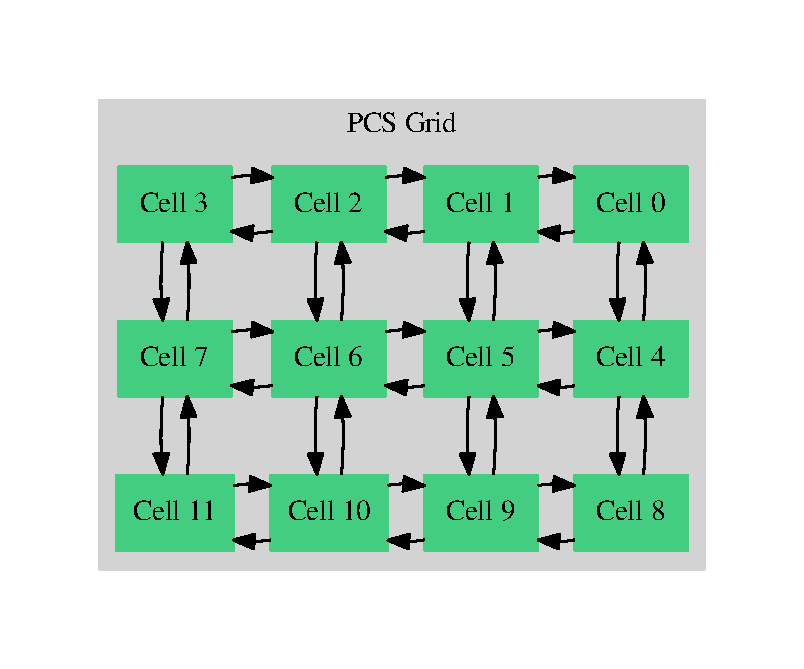
\includegraphics[width=0.6\textwidth]{figs/graphviz/pcs_model.pdf}
    \caption{PCS Model Logical Processes}\label{pcs_model_lps}
\end{figure}

State Variables:
\begin{itemize}
    \item Number of idle channels
    \item Number of call attempts
    \item Number of channel blocks
    \item Number of handoff blocks
\end{itemize}

\subsection{Traffic}

\begin{figure}[H]
    \centering
    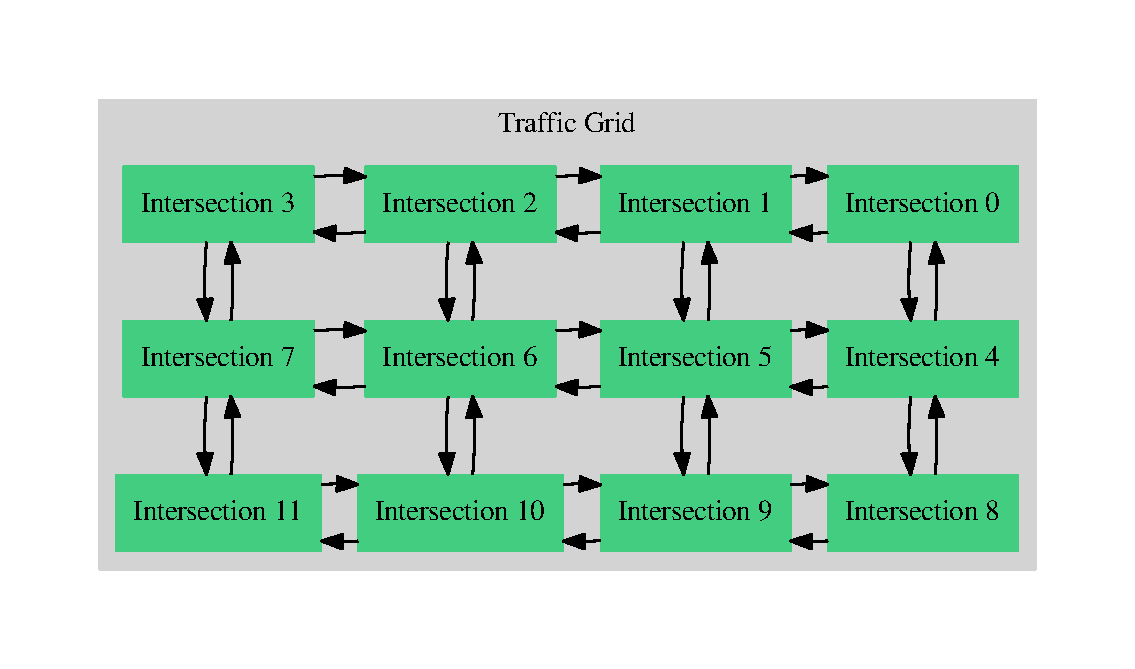
\includegraphics[width=\textwidth]{figs/graphviz/traffic_model.pdf}
    \caption{Traffic Model Logical Processes}\label{traffic_model_lps}
\end{figure}

\subsection{Epidemic}

\subsection{Airport}



\chapter{\textsc{warped2} Data Structures and Their Organization}\label{warped2_ds}

\section{Pending Event Set Data Structures}

The pending event set is the set of all unprocessed events. Every process contains a
logically seperate pending event set for a dedicated set of LPs. Exhanging of events
between LPs between processes is funneled through the manager thread of the processes.

Each LP has an unprocessed queue which contains both positive events and anti-messages and
remains sorted at all times. The anti-messages are given priority over their positive counterparts
to prevent any unnessary rolbacks and prevent cascading of rollbacks that can cause instability
\cite{lubachevsky-89}. To avoid any copying, the unprocessed queue only contains pointers
to the unprocessed events which are allocated by the simulation model. The worker threads
or manager thread send events to LPs by simply inserting the pointers into their unprocessed
queue.

A second type of data structure, an \emph{LTSF (Lowest TimeStamp First) Queue}, provides
order among events from multiple LPs. At most, a single event from each LP is \emph{scheduled}
into a single LTSF queue. Scheduling an event to an LTSF queue means only inserting a pointer
into the LTSF data structure with no removal from the unprocessed queue. The pending event
set contains one or more LTSF Queue to process events from.

A third type of data structure is also used to keep track of the events that have been
scheduled or are currently being processed and is organized by receiving LP. It is used for
two main reasons. First, it provides a way to determine if a smaller event is scheduled for
an LP upon the arrival of another event into its unprocessed queue. The new event can be
scheduled in place of the already scheduled event if that occurs. Second, it serves to
prevent multiple worker threads from processing events from the same LP which could cause
out of order committing of events violating the local causality constraint\cite{fujimoto-90}.

Figure \ref{pending_event_set} illustrates the pending event set data structures in
\textsc{warped2}.

\begin{figure}[H]
    \centering
    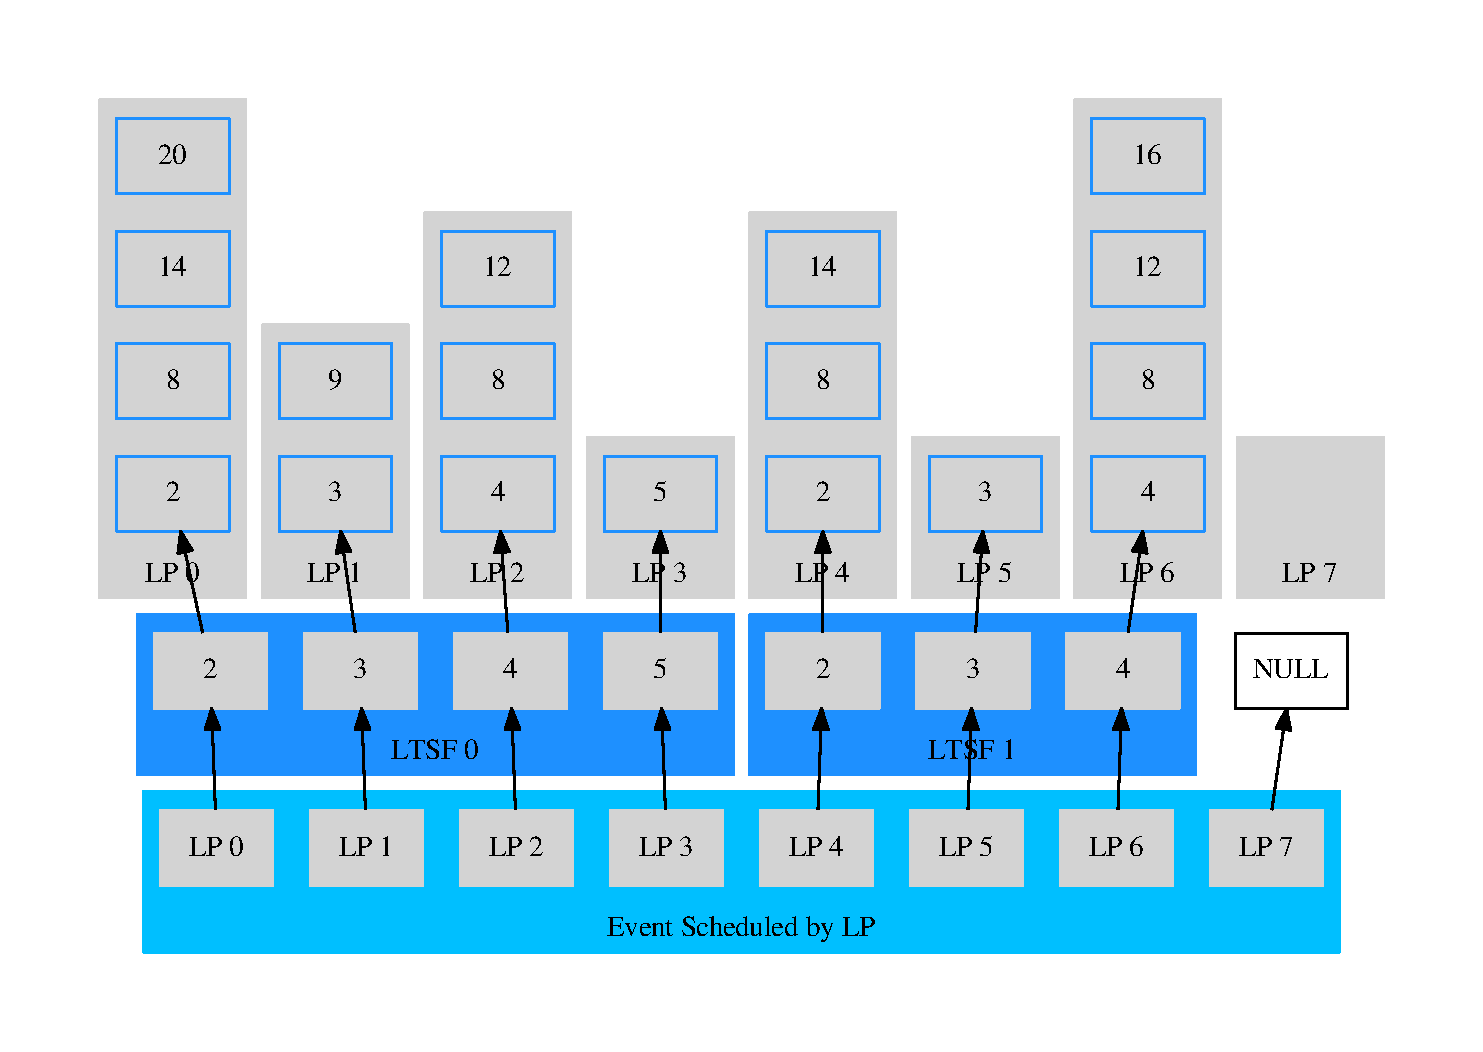
\includegraphics[width=0.75\textwidth]{figs/graphviz/pending_event_set.pdf}
    \caption{\textsc{warped2} Pending Event Set Date Structures}\label{pending_event_set}
\end{figure}

\section{Processing Events}

One or more of the worker threads are assigned to each LTSF Queue to process events from
and they all follow the exact same procedure. First, an event is removed from an LTSF
queue to be processed but remains in the unprocessed queue until it is processed. The
event is then checked to see if it is a straggler, and rolled back if so. An anti-message
is also considered a straggler if its positive counterpart was the last processed event
since \textsc{warped2} makes the assumption that events cannot be sent out of order.
If the event is an anti-message, the positive counterpart is assumed to be in the LPs
unprocessed queue after rolling back and is cancelled out and a new event is scheduled.
If the event is positive it is processed normally, the state of the LP is saved, and
new events are sent to other LPs. The event is then inserted into the processed queue
of the LP and a new event is scheduled if one exists for the LP. Lastly, the data structure
that keeps track of scheduled events by LP is updated. To summarize the worker thread
processing loop is shown in psuedocode in algorithm \ref{warped2_processing}.

\begin{algorithm}
\DontPrintSemicolon
\SetKw{Continue}{continue}
\SetKwFunction{getNextEvent}{getNextEvent}
\SetAlgoVlined

    \While{termination not detected}{
        \nlset{SQCRIT} $e \gets \getNextEvent{}$\;
        $lp \gets$ receiver of $e$\;\;

        \If{$e <$ last processed event for $lp$}{
            rollback $lp$\;
        }
        \;
        \If{$e$ is an anti-message}{
            cancel event with $e$\;
            \nlset{SQCRIT} schedule new event for $lp$\;
            \Continue\;
        }
        \;
        process event $e$\;
        save state of $lp$\;
        \nlset{SQCRIT} send new events\;
        \nlset{SQCRIT} replace scheduled event for $lp$\;
    }

\caption{\textsc{warped2} Main Event Processing Loop}\label{warped2_processing}
\end{algorithm}

When events are sent to an LP that is local to the process, they are directly inserted
into the unprocessed queue and checked against the currently scheduled event. If the
new event is less than the scheduled event, the scheduled event is replaced. When events
are sent to an LP that is not local to the process, they are inserted into a shared data
structure called the \emph{remote event queue}. The manager thread removes the events from
the remoted event queue, serializes them into messages and sends them to remote processes
through the communication manager.



\subsection{Total Ordering of Events}

The time warp system assumes that every event is labeled with a totally ordered clock value
based on virtual time \cite{jefferson-85}. This is important so that causal dependencies
are preserved and so that simulation results are deterministic\cite{ronngren-99}.
\textsc{warped2} uses a four tuple scheme which provide a total ordering of events:

\begin{enumerate}
    \item Receive Time
    \item Send Time
    \item Sender LP Name
    \item Generation
\end{enumerate}

\noindent
The last three serve as a tie breaker for simultaneous receive times. The send time is
necessary to ensure correct causal dependencies. It is analogous to a Lamport logical
clock\cite{lamport-78} in real time distributed systems but for virtual time systems. The
send time works for this as long as LPs only send a single event with the same send time
to any individual LP. The sender LP name is necessary to ensure that order is determined
between events received with the same receive time and send time from different senders.
Without it, it is possible that different results could occur on different runs of the
simulation\cite{ronngren-99}. The generation is necessary for distributed systems to
differentiate between the same events which could be resent after rolling back
\cite{ronngren-99}. In \textsc{warped2} it is implemented as a single counter per LP and
keeps track of the number of events that have been sent from the LP.

\subsection{Performance Analysis}

%%\showPlots{Schedule Queue Performance.pdf}{sq_performance}{Schedule Queue Performances}

\section{Data Structures to Support Rollback and Cancellation}

\begin{figure}[H]
    \centering
    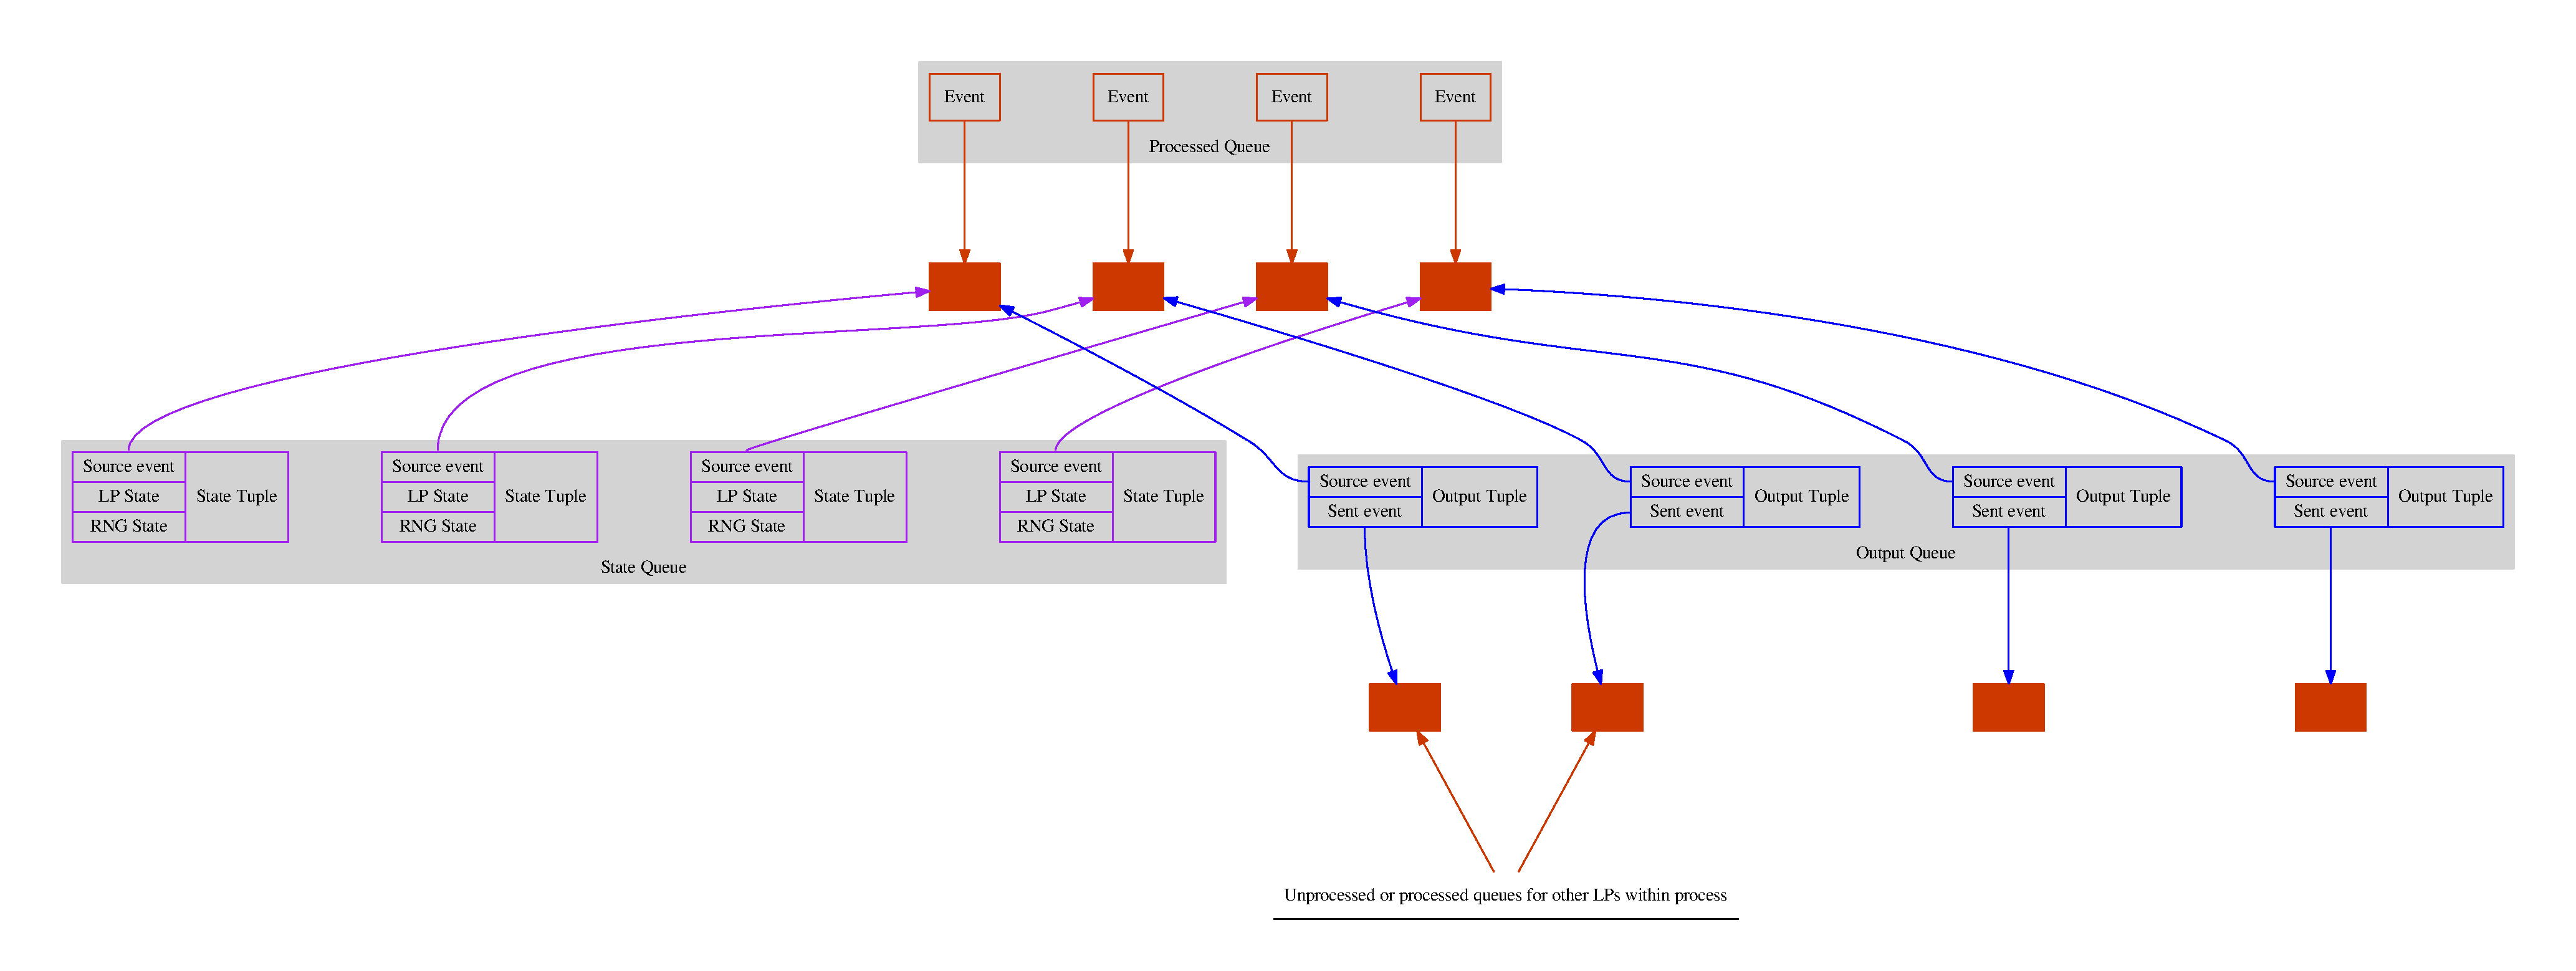
\includegraphics[width=\textwidth]{figs/graphviz/rollback_ds.pdf}
    \caption{Rollback and Cancellation Data Structures in \textsc{warped2}}\label{rollback_ds}
\end{figure}

\section{Protecting Access to Shared Data Structures}

\subsection{Performance Analysis}

\chapter{Partitioning}\label{partitioning}

\section{Overview}

Partitioning the work in a distributed system is always important to minimize interprocess
communication. In parallel discrete event simulation, the work is usually partitioned by
the LPs. Each process in the system can then process events from a dedicated subset of LPs.

In a message based system, communication latency is much larger than the frequency of
computation. The disparity of of communication time and compute time greatly increases
the chances of rollbacks occuring in a time warp system. Partitioning can greatly reduce
communication between processes, effictively pushing each process closer to a sequential
simulation.

In a shared memory system, partitioning can aid reducing the number of simulateous accesses
to shared data structures (e.g. unprocessed queues). Although it may not reduce the total
number of accesses to a data structure, it can force worker threads to access the same
subset of data structures reducing contention. This can also enhance the number of cache
hits by increasing locality.

\section{Partitioning in \textsc{warped2}}

Since \textsc{warped2} uses multiple worker threads within multiple processes, two levels
of partitioning is done. The first level of partitioning is for allocating LPs to processes
and the second level is for allocating LPs to an LTSF queue.

\subsection{Process Partitioning}



\subsection{LTSF Queue Partitioning}

Each process further partitions the LPs by the LTSF Queue that the LPs schedule their
events to. It is effectively partioning among worker threads if each worker thread has its
own LTSF Queue and has no effect if a single LTSF is shared among worker threads.


\chapter{GVT and Termination Detection}\label{gvt_termination}

Algorithms that compute the Global Virtual Time (GVT) and detect termination conditions are
both examples of algorithms that can be solved by determining the global state of a
distributed system. The global state of a system is defined as the combination of all
the local states of the processes in the system and all messages in transit. Global state
determination algorithms are also commonly used for deadlock detection, garbage collection,
debugging, and checkpointing for failure recovery in distributed systems.

\section{Global Snapshots}

\paragraph{Chandy and Lamport}\cite{chandy-85} described a basic global state algorithm by
using \emph{global snapshots} for distribtuted systems that use only FIFO channels for
communication. To start the algorithm, an initiator process records it's state and sends
a control token out of all outgoing channels. When a process receives a control token, and
it hasn't yet recorded its state, the process records its state and sends more control
tokens out of all its outgoing channels. The algorithm terminates at each process when it
has recieved a token through all of its incoming channels.

\paragraph{Lai and Yang}\cite{lai-87} describe an algorithm for non-FIFO systems which
computes a consistent cut by piggybacking a control bit onto basic messages. The control
bit is used to indicate whether or not the sending process has recorded its state. The
processes can be explained in terms of colors. A process that has not recorded its state
is colored white and a process that has recorded its state is red. White processes send
white messages and red processes send red messages. The control bit in the messages indicates
the color. All processes are initially white and turn red when a red message arrives. When
a red message arrives at a white process, the process must record its state BEFORE actually
receiving the message. The snapshot only relies on basic messages and no control tokens are
used. This algorithm has several drawbacks. First, it assumes that every process will
eventually receive a red message and record its state which is not guarenteed. Second, to
ensure transient messages are recorded, the processes must record all incoming and outgoing
messages and send them to other processes within the basic messages. That way the transient
messages can be calculated by differences in incoming and outgoing messages.

\paragraph{Mattern}\cite{mattern-93} extended the algorithm by Lai and Yang by adding a
seperate control token which is used to create two cuts by cirulating the control token to
every process twice. The control token is used to color the processes instead of the basic
messages. This guarentees that every process will eventually record its state because the
token is always circulated. Furthermore, processes do not have to keep track of sent and
received messages. Instead counters can be used to keep track of the differences in sent
and received white messages at each process. The control token can then accumulate the
counts. When the white message counts accumulate to zero when the token arrives back at
the initiator proccess, it can be determined that the snapshot is complete. These counters
can be \emph{vector counters} or \emph{scalar counters}. Vector counters keep track of
messages to/from each process individually whereas scalar counters keep track of just a
single count at each process. When the algorithm is complete, only the initiator process
can produce a global snapshot so if all processes must use the snapshot, it must be broadcasted
to the other processes.

\section{GVT}

Although GVT algorithms can be implemented with the basic global snapshot algorithms described
above, it is usually more efficient to build custom solutions on top of the basic algorithms.
In a GVT algorithm, the local minimum clock of process is the local state and the basic
messages are events that are sent between processes. This section first describes the key
ideas that must be considered when developing a GVT algorithm. Then, a few of the classic
GVT algorithms and modern GVT algorithms that are commonly used in practice today are described.
Finally, the algorithm that is implemented in \textsc{warped2} is described as well as the
reasons for choosing the approach.

GVT algorithms can be synchronous or asynchronous. In a synchronous GVT algorithm, since
all other computation will be blocked, event processing will be halted. Synchronous GVT
algorithms are usually very simple to implement but halting the event processing can
be very costly. On the other hand, asynchronous GVT algorithms calculate GVT concurrently
with event processing. For this reason, asynchronous GVT algorithms perform much better
than synchronous GVT algorithms but are harder to implement because special cases must be
considered.

There are two special cases that must be considered in any GVT algorithms:

\begin{description}
    \item[Transient Message Problem:] is caused by messages(events) that have been sent by
    the sending process but not yet recieved by the receiving process. If not carefully
    considered in a GVT algorithm, these \emph{transient messages} can be completely missed
    which could lead to an erroneous GVT calculation if they contain the minimum timestamp
    of all other events in the system.
    \item[Simultaneous Reporting Problem:] is caused because processes can report their local
    minimum clock at different points in real time. Consideration must be taken into account
    to ensure that a process does not report its local minimum clock value and then receive
    an event from a process that has not yet reported its local minimum clock value,
    completely missing the event.
\end{description}

\noindent
There are many synchronous and asynchronous GVT algorithms that have been developed over the
years that all have some method of either solving these problems.

\subsection{Asynchronous GVT Algorithms}

\subsubsection{Message Passing Algorithms}

Most of the time warp systems in use today are based on message passing and classically
GVT algorithms have been designed for message passing systems. In this section Samadi's and
Mattern's message passing algorithms are discussed and in the next section Fujimoto's shared
memory GVT algorithms is discussed as well as the Seven O'Clock algorithm which is an
extension of Fujimoto's shared memory algorithm extended for distributed memory systems.

\paragraph{Samadi's Algorithm}\cite{samadi-85} in the most general form uses acknowledgements
for all events that have been received. All processes must track all events that have been
sent but have not been acknowledged. Furthermore, the received messages must also be tracked
so that acknowlegements can be sent. All transient message can then be calculated from the
tracked messages. A process initiates the GVT algorithm by broadcasting a start message to
all processes. After this start message is received by a process, it is marked(colored) and
all acknowledgements sent from a marked process are also marked(colored). All processes then
calculate their local minimum by taking the minimum of the unacknowledged received events,
the marked acknowledgments sent, and the local simulation clock. Marking the acknowledgements
sent after the start of the GVT calculation ensures that the simultaneous reporting problem
will not occur.

\paragraph{Mattern's Algorithm}\cite{mattern-93} for GVT calculation is an extension on his
general snapshot algorithm that was described above. The white message counts are used to
determine whether transient messages are still in the sytem. They also serve as the basis
for determining when the snapshot is complete which occurs when the accumulated white message
count of all processes is zero. To ensure that the simultaneous reporting problem does not
occur, red messages received at a white process are recorded and used in the local minimum
value. The algorithm is initiated by sending a control token to all processes in some defined
order. The token accumulates the white message counters, local minimum clocks, and minimum
red message timestamps. When the accumulated count reaches zero and the token is back at
the initiator process, the GVT is approximated using the minimum of the accumulated clocks
and timestamps.

\paragraph{Other GVT Algorithms} that are based on message passing model are usually based
on the same ideas from Samadi's algorithm or Mattern's algorithm. Many algorithms are just
extensions or variations of the algorithms that aim to optimize it in some particular way.

\subsubsection{Shared Memory Algorithms}

\paragraph{Fujimoto's Algorithm}\cite{fujimoto-94} is a fast GVT algorithm that exploits
properties of shared memory architectures. In most shared memory architectures, processors
cannot observe memory operations in different orders. For this reason, it is not possible
to have transient messages if a shared data structure is used to communicate between tasks
running on different processors. Furthermore, a shared flag variable can be used to initiate
the GVT algorithm. However, it is still possible that the flag can be read at different
times, so the simultaneous reporting problem can still occur. To solve the simultaneous
reporting problem, two things must be done, First, the start flag is checked after sending
events and recorded if the sending task has not yet reported its local minimum value and
is eventually used when the reporting is done. Second, the start flag must be read into a
temporary local variable before obtaining a new event to process.

\paragraph{Seven O'Clock Algorithm}\cite{bauer-05} is an extension of Fujimoto's algorithm
for distributed memory systems. Although the algorithm can be used in message passing systems,
the algorithm does not use any messages and is still uses shared memory ideas. The key idea
in the algorithm is that all processors in a distributed system all have a consistent view
of wall clock. Hence, the processors can carry out an operation atomically, without having
to explicitly interact. The atomicity can be achieved by using cycle level counters which
are available on most modern architectures. Unlike Fujimoto's algorithm though, transient
messages can still be missed in the calculation. To solve that problem, each processor must
wait a small time interval which is calculated based on the worst round trip time for
network transactions.

\subsection{Synchronous GVT Algorithms}

\paragraph{Global Reductions} provide a good way to do a synchronous minimum calculation
which and is a common way to implement a synchronous GVT algorithm. ROSS implements a
synchronous GVT algorithm which uses global reductions\cite{holder-08}. First, to prevent
the transient message problem, a global reduction on message counts of each process is
performed until it reaches zero which is guarenteed because the reduction acts as a barrier
for each process. The message counting is necessary because asynchronous communication is
used for sending and receiving events. When the messages count reaches zero a global
reduction is performed on the local minimum timestamp of all processes to give a GVT value
which is broadcast to all processes. This algorithm is efficient when time warp simulation
are run on large supercomputing platforms like the blue gene machine which perform collective
operations very quickly.

\subsection{Warped2 Algorithm}

To calculate the GVT in \textsc{warped2}, Fujimoto's shared memory algorithm is used between
worker threads and a variation of Mattern's algorithm with scalar message counters is used
between processes. Hence, Fujimoto's algorithm is a subalgorithm of Mattern's algorithm.
The details of the Mattern's algorithm implementation in \textsc{warped2} is detailed below
as well as how it is used with Fujimoto's algorithm.

In the \textsc{warped2} implementation, scalar counters are used to keep track of message
that are sent that carry the initial color. That means that each process keeps track of
the number of sent messages minus the number of received messages to and from all other
process as a single counter. The reason that scalar counters are used over vector counters
is that vector counters require that communication is stopped after receiving a control token
until all known transient messages bound for the receiving process are received. With scalar
counters, this is not possible because it is only a single counter. However, it is possible
that more than two rounds of the control token will be necessary. This is usually not a
problem in practice though since two rounds is usually sufficient. With scalar counters,
each process must maintain a counter for both white messages \emph{and} red messages so
that counters can be consistent between multiple runs of the algorithm. Moreover, the role
of colors must be switched between successive runs.

In the description of the \textsc{warped2} algorithm, the colors will be described as
\emph{initial} and \emph{final}. Each process also keeps track of its current color, a
minimum timestamp of an event received with the final color, and temporary variables to
hold accumulated values from the token. The variables that are maintained at each
process and are used in the succeeding discussion are listed below in algorithm
\ref{process_variables}.

\begin{algorithm}
\DontPrintSemicolon
    \boldmath$ts_{min}:$ Minimum timestamp of event messages received with final color\;
    \boldmath$color:$ Current color of the process\;
    \boldmath$color_{initial}:$ Intial color of all processes\;
    \boldmath$msgcount_{initial}:$ Messages sent minus messages received with initial color\;
    \boldmath$msgcount_{final}:$ Messages sent minus messages received with final color\;
    \boldmath$clock_{min}:$ Temporary variable to hold accumulated minimum clock from all
        processes\;
    \boldmath$msgcount:$ Temporary variable to hold accumulated initial color message count
        from all processes\;
\caption{Process Variables in \textsc{warped2} Mattern Implementation}\label{process_variables}
\end{algorithm}

\noindent
The event messages that are sent between processes contain the format:

    $<sender, receiver, mcolor,...>$

\noindent
where $sender$ is the id of the sender process, $receiver$ is the id of the reciever process,
and $mcolor$ is the color of the message. The message color is the color of the sending
process at the time it is sent. The message count for the current color is also incremented
when it is sent. Psuedocode illustrating this procedure is shown in algorithm \ref{gvt_event_send}.

\begin{algorithm}
\DontPrintSemicolon
\SetAlgoVlined
    $mcolor \gets color$\;
    \If {$color = color_{initial}$} {
      $msgcount_{initial} \gets msgcount_{initial} + 1$\;
    }
    \Else {
      $msgcount_{final} \gets msgcount_{final} + 1$\;
    }
\caption{Event Message Send}\label{gvt_event_send}
\end{algorithm}

When an event is received by a process the message count for the current color of the process
is decremented. If the color carried by the message is the final color in the algorithm,
indicating that the sender has already reported a local minimum value, then the timestamp
of the event is recorded as $ts_{min}$. Psuedocode illustrating the receiving procedure is
show in algorithm \ref{gvt_event_receive}.

\begin{algorithm}
\DontPrintSemicolon
\SetAlgoVlined
    \If{$color_{message} = color_{initial}$} {
        $msgcount_{initial} \gets msgcount_{initial} - 1$\;
    }
    \Else {
        $msgcount_{final} \gets msgcount_{final} - 1$\;
        $ts_{min} \gets \min{(ts_{min}, ts_{event})}$\;
    }
\caption{Event Message Receive}\label{gvt_event_receive}
\end{algorithm}

\noindent
The control token that is sent between processes contains the format:

    $<sender, receiver, mclock, msend, mcount>$

\noindent
where $mclock$ is an accumulated minimum of all local minimum clocks at all processes
visited by the token, $msend$ is an accumulated minimum of all $ts_{min}$ values at all
processes visited by the token, and $mcount$ is an accumulated sum of $msgcount_{final}$
from all processes visited by the token.

In the \textsc{warped2} implementation, the token is passed in logical ring fashion to
increasing process ids and is initiated by process with id 0. When the token reaches
process $N-1$, where $N$ is the number of processes in the system, it is sent back to
process 0. To start the algorithm, process 0 toggles its color, resets minim values to
infinity, stores the initial color message count into a temporary variable $msgcount$, and
starts Fujimoto's algorithm. When Fujimoto's algorithm is complete, it will send the token
$<0, 1, lvt_{min}, ts_{min}, msgcount>$ with $lvt_{min}$ being the result of Fujimoto's
algorithm. Psuedocode illustrating the start procedure is shown in algorithm \ref{gvt_start}.

\begin{algorithm}
\DontPrintSemicolon
\SetAlgoVlined
\SetKwFunction{SendToken}{SendToken}
\SetKwFunction{Fujimoto}{doFujimoto}
    \If{$color = WHITE$}{
        $color \gets RED$\;
    } \Else {
        $color \gets WHITE$\;
    }
    $ts_{min} \gets \infty$\;
    $clock_{min} \gets \infty$
    $msgcount \gets msgcount_{initial}$\;
    $msgcount_{initial} \gets 0$\;
    $lvt_{min} \gets \Fujimoto{}$\;
    \SendToken{$0, 1, lvt_{min}, ts_{min}, msgcount$}\;
\caption{Mattern Algorithm Start Procedure}\label{gvt_start}
\end{algorithm}

When a token is received at a process that is not the initiator and it still has the initial
color then the color is toggled. Then, the minimum timestamp received from final colored
messages, the minimum clock value, and the initial message count for the process are
accumulated with the token's value. The initial message count is then reset so it will not
be used in the next round and Fujimoto's algorithm is initiated. When Fujimoto's algorithm
is completed, the token is sent to the next process with all of the accumulated values
including $lvt_{min}$ calculated from Fujimoto's algorithm. This procedure is illustrated
in psuedocode shown in algorithm \ref{gvt_receive_noninit}.

\begin{algorithm}
\DontPrintSemicolon
\SetAlgoVlined
\SetKwFunction{SendToken}{SendToken}
\SetKwFunction{Fujimoto}{doFujimoto}
    \If{$color = color_{initial}$} {
        $ts_{min} \gets \infty$\;
        \If{$color = WHITE$}{
            $color \gets RED$\;
        } \Else {
            $color \gets WHITE$\;
        }
    }
    $ts_{min} \gets \min{(ts_{min}, msend)}$\;
    $clock_{min} \gets \min{(clock_{min}, mclock)}$\;
    $msgcount \gets msgcount_{initial} + msgcount$\;
    $msgcount_{initial} \gets 0$\;
    $lvt_{min} \gets \Fujimoto$\;
    \SendToken{$i, (i+1) \bmod N, \min{(lvt_{min}, clock_{min})}, ts_{min}, msgcount$}\;
\caption{Mattern Control Token Receive Procedure: Non-initiator Node}\label{gvt_receive_noninit}
\end{algorithm}

When a token is received at a the initiator process, it can be assumed that a minimum clock
value has already been included in the token that is received. If the accumulated message count
for the initial color has reached zero, then the GVT can be appoximated and the algorithm
is terminated. If there are still transient message that were not accounted for, the initiator
process initiates a new round until the resulting message count accumulation is zero
when received at the initiator. The GVT is approximated at the initiator by taking the
minimum of the accumulated minimum clock values and the accumulated minimum timestamp values
and broadcast to the rest of the processes. This procedure is illustrated in the psuedocode
in algorithm \ref{gvt_receive_init}.

\begin{algorithm}
\DontPrintSemicolon
\SetAlgoVlined
\SetKwFunction{SendToken}{SendToken}
\SetKwFunction{Fujimoto}{doFujimoto}
\SetKwFunction{SendGVTUpdate}{SendGVTUpdate}
    \If {$mcount = 0$} {
        $gvtApprox \gets \min{(mclock, msend)}$\;
        \SendGVTUpdate{}\;
        \If{$color_{initial} = WHITE$}{
            $color_{initial} \gets RED$\;
        } \Else {
            $color_{initial} \gets WHITE$\;
        }
        $clock_{min} \gets \infty$\;
    } \Else {
        $ts_{min} \gets \min{(ts_{min}, msend)}$\;
        $msgcount \gets msgcount_{initial} + mcount$\;
        $msgcount_{initial} \gets 0$\;
        $lvt_{min} \gets \Fujimoto$\;
        \SendToken{$i, (i+1) \bmod N, lvt_{min}, ts_{min}, msgcount$}\;
    }
\caption{Mattern Control Token Receive Procedure: Initiator Node}\label{gvt_receive_init}
\end{algorithm}

\section{Termination Detection}

Termination detection, like GVT, is a problem of determining the global state of the system.
Termination is a \emph{stable property} of a distributed system, meaning that once termination
conditions occur, the system will remain with termination conditions forever until further
action is taken.

A process in the system can be in one of two states at any time: active or passive. A process
is considered active if some basic computation still remains and passive otherwise.
When all processes in the system become passive and no messages are left in transit, then
the system should be terminated. The purpose of the termination detection algorithm is to
determine when this occurs. A passive process can become active with the arrival of an
\emph{activation message}. For parallel discrete event simulation the basic computation is
event processing and the activation messages are events. A termination detection for any
parallel discrete event simulation must satisfy the following properties:

\begin{description}
    \item[Safety:] Termination will not be detected if any unprocessed event is still present
        in system including all local pending event sets and events still in transit.
    \item[Liveness:] Termination will be detected at some finite amount of time after all
        events have been processed.
\end{description}

Just like GVT algorithms, termination detection algorithms can implemented with message
passing or shared memory. Termination algorithms vary widely because different systems
can define termination conditions in such different ways. Furthermore, termination usually
does not affect system performance so correctness is more important than optimization.
For these reasons only the termination algorithm that is implemented in \textsc{warped2}
will be discussed any further. It is actually two independant algorithms, a message passing
algorithm and a shared memory algorithm. In the opposite manner as the GVT algorithm, the
shared memory algorithm is actually used to initiate the message passing algorithm.

\subsection{Shared Memory algorithm}

The purpose of the shared memory algorithm is to determine when all of the worker threads
in a process become passive (inactive). The algorithm is fairly straightforward and uses
just a single shared counter variable to keep track of the number of active worker threads
and a boolean array to keep track of which worker threads are active. Worker threads can
only read or write to their own status values. The counter is updated atomically to avoid
possible race condtions.

The safety property is achieved because there can be no transient messages. If a thread
sends an event to an LP that will be processed by another thread and then becomes inactive,
false termination cannot detected because the receiving thread becomes active again after
seeing the event. Come back to this, it may not be accurate.
The liveness property is achieved because the manager thread periodically checks the
active worker thread count so the inactivity of all worker threads will eventually be
discovered. If the count is zero, then the message passing algorithm will be initiated
between processes.

\subsection{Message Passing Algorithm}

The algorithm that is carried out among processes is an asynchronous message passing
algorithm based on Mattern's "sticky flags" algorithm\cite{mattern-93}. Just like the GVT
algorithm, the token is passed in a logical ring to increasing process ids. However, the
initiator process of the algorithm is dynamic. The initiator is the first active process
that the token reaches during circulation. For the first circulation, the initator is process
0.

Each process has two states, one for the actual state and one for the \emph{sticky state}.
The sticky state is the state that is actually used in the algorithm. It becomes active
when the actual state becomes active but sticks to active when the actual state becomes
passive. The sticky state can only changes to passive on the arrival of a token. By using
this scheme the token is forced to circulate two times with no process becoming active and
ensures the safety property. Without this scheme, a process that has already forwarded the
token because it was passive could receive an activation message and then the sender of the
activation message could become passive before receiving the token. False termination could
then be detected.

The process variable names that are used for the succeeding discussion are listed in
algorithm \ref{termination_variables}.

\begin{algorithm}
\DontPrintSemicolon
    \boldmath$state_{actual}:$ Indicates the actual state of the process at all times\;
    \boldmath$state_{sticky}:$ Indicates the state of the process if active, but may stick
        to active if passive\;
    \boldmath$initiator:$ Boolean variable indicating process is leader\;
\caption{Process Variables in Termination Detection Algorithm}\label{termination_variables}
\end{algorithm}

\noindent
The termination token that is sent between process has the format:

    $<sender, receiver, mstate, minitiator>$

\noindent
where $sender$ is the id of the sending process, $receiver$ is the id of the receiving
process, $mstate$ is the partial state of system based on visited processes, and $minitiator$
is the process id of the initiator.

The algorithm is started when the initiator process becomes passive which is determined by
the shared memory algorithm. When a process receives the token it becomes the initiator
but loses its roles as initiator when it sends the token. That way, only a single process
can be the initiator. Furthermoe, since the token always stops at an active process, the
token is always guarenteed to start again when it becomes passive which also guarentees
the liveness property. When the token is received back at the initiator with a passive
state, then termination is signaled to all processes. The procedure is illustrated in
algorithm \ref{termination_token_receive}.

\begin{algorithm}
\DontPrintSemicolon
\SetAlgoVlined
\SetKw{And}{ and }
\SetKwFunction{SendToken}{SendToken}
    $initiator \gets true$\;
    \If{$state_{sticky} = PASSIVE \And state_{process} = minitiator$} {
        \If{$mstate = PASSIVE$} {
            Signal termination\;
        }
    } \ElseIf{$state_{sticky} = PASSIVE$} {
        $initiator \gets false$\;
        \SendToken{$mstate, minitiator$}\;
    }
    $state_{sticky} \gets state_{actual}$\;
\caption{Termination Token Receive Procedure}\label{termination_token_receive}
\end{algorithm}

It should also be noted that this algorithm is only guarenteed to work if the message order
is preserved. If that is not the case, then message counters are necessary to ensure
transient activation messages are not missed.

\chapter{Memory Management}\label{memory_management}

This chapter will focus on three main topics that are all related to the management
of memory. First, state saving techniques will be discussed as well the analysis of state
saving in \textsc{warped2}. This will include both space and time requirements. Then fossil
collection and its overheads are introduced and a comparison of worker thread versus manager
thread fossil collection will be examined. Lastly, memory allocation and deallocation and
its importance in time warp is presented as well as how it is accomplished in \textsc{warped2}.

\section{State Saving}

\paragraph{Copy-state Saving} is the classic state saving technique that saves every past
state of every LP and requires that the all states are copied and saved into the state queues.
This method requires a lot of extra memory and requires a lot of extra computation to copy
the states and insert them into the state queue. For this reason, copy-state saving is
usually used in conjuction with other technique or not at all.

\paragraph{Periodic State Saving} is another state saving technique where the state of each LP
is saved only once every N events, where N is a number greater than one. Periodic state
saving can significantly reduce the overhead of the time taken to copy the state of the
LPs into the state queue. However, due to state history being lost, more processed event
have to be saved so that the state of LPs can be restored correctly. These saved events
must be reprocessed to restore the state in a process known as \emph{coast forwarding}.
During coast forwarding the events are processed normally but only to update the state.
The only difference is that no events are sent during the coast forwarding phase. The
downside is that the rollback length is increased due to the loss in state saving. However,
periodic state saving is a significant improvement over the base copy-state staving approach
since the reduced time in state saving far outweighs the extra rollback time for increased
rollback length.

\paragraph{Incremental State Saving} is a technique that aims to reduce the amount of
memory needed to store past states of the LPs. Instead of saving entire snapshots of the
past states, the differences in specific state variables are saved. This method requires
that metadata describing which variables are modified for each event. Therefore, this approach
works well as long as only a small portion of the state variables change during the forward
execution of events.

\paragraph{Reverse Computation} is a modern approach to state state saving that does not
actually save any past states of the LPs. Instead, the \emph{control state} of the forward
computation is saved as a set of bits that describe the control flow. By saving the control
flow of the forward execution for each event, the state variables that are modified and
how they are modified are known and can be reversed. That is, at least, if all state variables
are reversible without the need to know the histories of the variables. Also, a reversible
random number generator is required. These are both practical requirements, though. The major
problem with this approach is the necessity to understand forward and reverse computation
precisely in the implementation of the simulation model.

\subsection{State Saving Experimental Assessment}

\textsc{warped2} currently implements only periodic state saving because it works well
regardless of the simulation model and it can be implemented transparently in the simulation
kernel.

%% State saving period analysis
%%\showPlots{State Saving Performance.pdf}{ssp_performance}{State Saving Performances}

\section{Fossil Collection}



\paragraph{GVT-based Fossil Collection}

\paragraph{On-the-fly Fossil Collection}

\paragraph{Optimistic Fossil Collection}

\subsection{Fossil Collection Experimental Assessment}

%% Manager thread versus Worker Threads

\section{Memory Allocation}

\subsection{Thread-Caching Malloc (TCMalloc)}

\chapter{Observations with the ARM big.LITTLE Platform}

\section{}

\chapter{Summary of Results}\label{results_summary}

%% DOUG: wrap up the results, review the main configurations that make sense to the best
%% general performance that one could expect to use.  depending on your principle results,
%% this may have to be broken down into two main parts, one for x86 and one for ARM.

\chapter[Conclusions \& Future Research]{Conclusions and Suggestions for Future Research}
\label{conclude}

\section{Summary of Findings}

\section{Detailed Conclusions}

\section{Suggestions for Future Work}

%%\Appendix
%%\chapter{Appendix A}\label{appendixA}


\bibliography{refs}
\bibliographystyle{ieeetr} \markright{ }

\end{document}
